\documentclass{article}
\usepackage[left=4cm, right=4cm, top=3cm, bottom=3cm]{geometry}
\usepackage{amsmath}
\usepackage{hyperref}
\DeclareMathOperator*{\argmax}{\arg\!\max}
\usepackage{amssymb}
\usepackage[utf8]{inputenc}
\usepackage{graphicx}
\graphicspath{{../images/}}
\usepackage{csquotes}
\setlength{\parindent}{0cm}
\usepackage[font={small, it}]{caption}

\newcommand\RepoAddress{https://github.com/enjeeneer/sutton_and_barto}
\newcommand\ProgrammingExercise{This is a programming exercise, the relevent code can be found on \href{\RepoAddress}{my GitHub}.}
\setcounter{tocdepth}{2}
\setcounter{secnumdepth}{1}

\title{Reinforcement Learning: An Introduction - Exercises}
\author{Scott Jeen}
\date{\today}

\begin{document}
	
	\maketitle
	\tableofcontents
	\section{Introduction}
\subsection{Exercise 1.1}
\subsubsection*{Q}
Suppose, instead of playing against a random opponent, the reinforcement learning algorithm described above played against itself, with both sides learning. What do you think would happen in this case? Would it learn a different policy for selecting moves?
\subsubsection*{A}
\textit{skipped}
$
\hfill \blacksquare
$

\subsection{Exercise 1.2}
\subsubsection*{Q}
Many tic-tac-toe positions appear different but are really the same because of symmetries. How might we amend the learning process described
above to take advantage of this? In what ways would this change improve the learning process? Now think again. Suppose the opponent did not take advantage of symmetries. In that case, should we? Is it true, then, that symmetrically equivalent positions should necessarily have the same value?
\subsubsection*{A}
\textit{skipped}
$
\hfill \blacksquare
$

\subsection{Exercise 1.3}
\subsubsection*{Q}
Suppose the reinforcement learning player was greedy, that is, it always played the move that brought it to the position that it rated the best. Might it learn to play better, or worse, than a nongreedy player? What problems might occur?
\subsubsection*{A}
\textit{skipped}
$
\hfill \blacksquare
$

\subsection{Exercise 1.4}
\subsubsection*{Q}
Suppose learning updates occurred after all moves, including exploratory moves. If the step-size parameter is appropriately reduced over time (but not the tendency to explore), then the state values would converge to a different set of probabilities. What (conceptually) are the two sets of probabilities computed when we do, and when we do not, learn from exploratory moves? Assuming that we do continue to make exploratory moves, which set of probabilities might be better to learn? Which would result in more wins?
\subsubsection*{A}
\textit{skipped}
$
\hfill \blacksquare
$

\subsection{Exercise 1.5}
\subsubsection*{Q}
Can you think of other ways to improve the reinforcement learning player? Can you think of any better way to solve the tic-tac-toe problem as posed?
\subsubsection*{A}
\textit{skipped}
$
\hfill \blacksquare
$
	\section{Multi-arm Bandits}
\subsection{Exercise 2.1}
\subsubsection*{Q}
In \(e\)-greedy action selection, for the case of two actions and \(e\) = 0.5, what is the probability that the greedy action is selected?

\subsubsection*{A}
Greedy action selected with \(p\) = 0.5
$
\hfill \blacksquare
$

\subsection{Exercise 2.2}
\subsubsection*{Q}
Bandit example Consider a k-armed bandit problem with k = 4 actions, denoted 1, 2, 3, and 4. Consider applying to this problem a bandit algorithm using \(e\)-greedy action selection, sample-average action-value estimates, and initial estimates of \(Q_1(a)\) = 0, for all \(a\). Suppose the initial sequence of actions and rewards is $A_1 = 1, R_1 = 1, A_2 = 2, R_2 = 1, A_3 = 2, R_3 = 2, A_4 = 2, R_4 = 2, A_5 = 3, R_5 = 0$. On some of these time steps the \(e\) case may have occurred, causing an action to be selected at random. On which time steps did this definitely occur? On which time steps could this possibly have occurred?

\subsubsection*{A}
\begin{table}[h!]
	\begin{tabular}{lllllll}
		\hline
		Timestep & \(Q_1\) & \(Q_2\) & \(Q_3\) & \(Q_4\) & Greedy action at timestep & Action selected \\  \hline
		0        & 0    & 0    & 0    & 0    & -                         & \(A_1\)     \\        \hline
		1        & 1    & 0    & 0    & 0    & \(A_1\)                      & \(A_2\)      \\       \hline
		2        & 1    & 1    & 0    & 0    & \(A_1/A_2\)                 & \(A_2\)      \\       \hline
		3        & 1    & 1.5  & 0    & 0    & \(A_2\)                      & \(A_2\)     \\        \hline
		4        & 1    & 1.66 & 0    & 0    & \(A_2\)                      & \(A_5\)    \\         \hline
		5        & 1    & 1.66 & 0    & 0    & \(A_2\)                      & end       \\       \hline
	\end{tabular}
	\label{table: ex2.2}
	\caption{Greedy actions at each timestep of a 4-armed bandit problem}
\end{table}
\begin{itemize}
	\item Action selection at timesteps 0, 1 and 4 are random as they are not reward maximising - see Table \ref{table: ex2.2}.
	\item Action selection at timestep 2 could be random as \(A_1\) is also reward maximising - see Table \ref{table: ex2.2}.
\end{itemize}
$
\hfill \blacksquare
$

\subsection{Exercise 2.3}
\subsubsection*{Q}
In the comparison shown in Figure \ref{fig:chapter2_2}, which method will perform best in the long run in terms of cumulative reward and probability of selecting the best action? How much better will it be? Express your answer quantitatively.

\subsubsection*{A}
In the limit of \(t \rightarrow \infty\), both non-zero \(e\)-greedy policies will learn the optimal action abd value function \(q*\). The policy with \(e\) = 0.01 will select the optimal action 10x more regularly than the policy with \(e\) = 0.1.
$
\hfill \blacksquare
$

\subsection{Exercise 2.4}
\subsubsection*{Q}
If the step-size parameters, \(\alpha_n\), are not constant, then the estimate \(Q_n\) is a weighted average of previously received rewards with a weighting different from that given by (2.6). What is the weighting on each prior reward for the general case, analogous to (2.6), in terms of the sequence of step-size parameters?.

\subsubsection*{A}
For a n-dependent \(\alpha\) we have:
\begin{align}
	Q_{n+1} &= Q_n +\alpha_n \left[R_n - Q_n\right] \nonumber \\
	&= \alpha_n R_n + (1-\alpha_n) Q_n\nonumber \\
	&= \alpha_n R_n + (1-\alpha_n) \left[Q_{n-1} + \alpha_{n-1} \left[R_{n-1} - Q_{n-1} \right]\right]\nonumber \\
	&= \alpha_n R_n + \alpha_{n-1} R_{n-1} - \alpha_n \alpha_{n-1} R_{n-1} + (1-\alpha_n)(1-\alpha_{n-1}) Q_{n-1} \nonumber \\
	&= \vdots \nonumber \\
	&= \sum_{i}^{n} \alpha_n R_n - R_{n-1} \prod_{i}^{n} \alpha_n + Q_{1} \prod_{i}^{n}(1-\alpha_n) \\
\end{align}
$
\hfill \blacksquare
$

\subsection{Exercise 2.5}
\subsubsection*{Q}
Design and conduct an experiment to demonstrate the difficulties that sample-average methods have for nonstationary problems. Use a modified version of the 10-armed testbed in which all the \(q_*(a)\) start out equal and then take independent random walks (say by adding a normally distributed increment with mean 0 and standard deviation 0.01 to all the \(q_*(a)\)  on each step). Prepare plots like Figure 2.2 for an action-value method using sample averages, incrementally computed, and another action-value method using a constant step-size parameter, \(\alpha\) = 0.1. Use \(\alpha\) = 0.1 and longer runs, say of 10,000 steps.

\subsubsection*{A}
\ProgrammingExercise
\begin{figure}[h!]
	\centering
	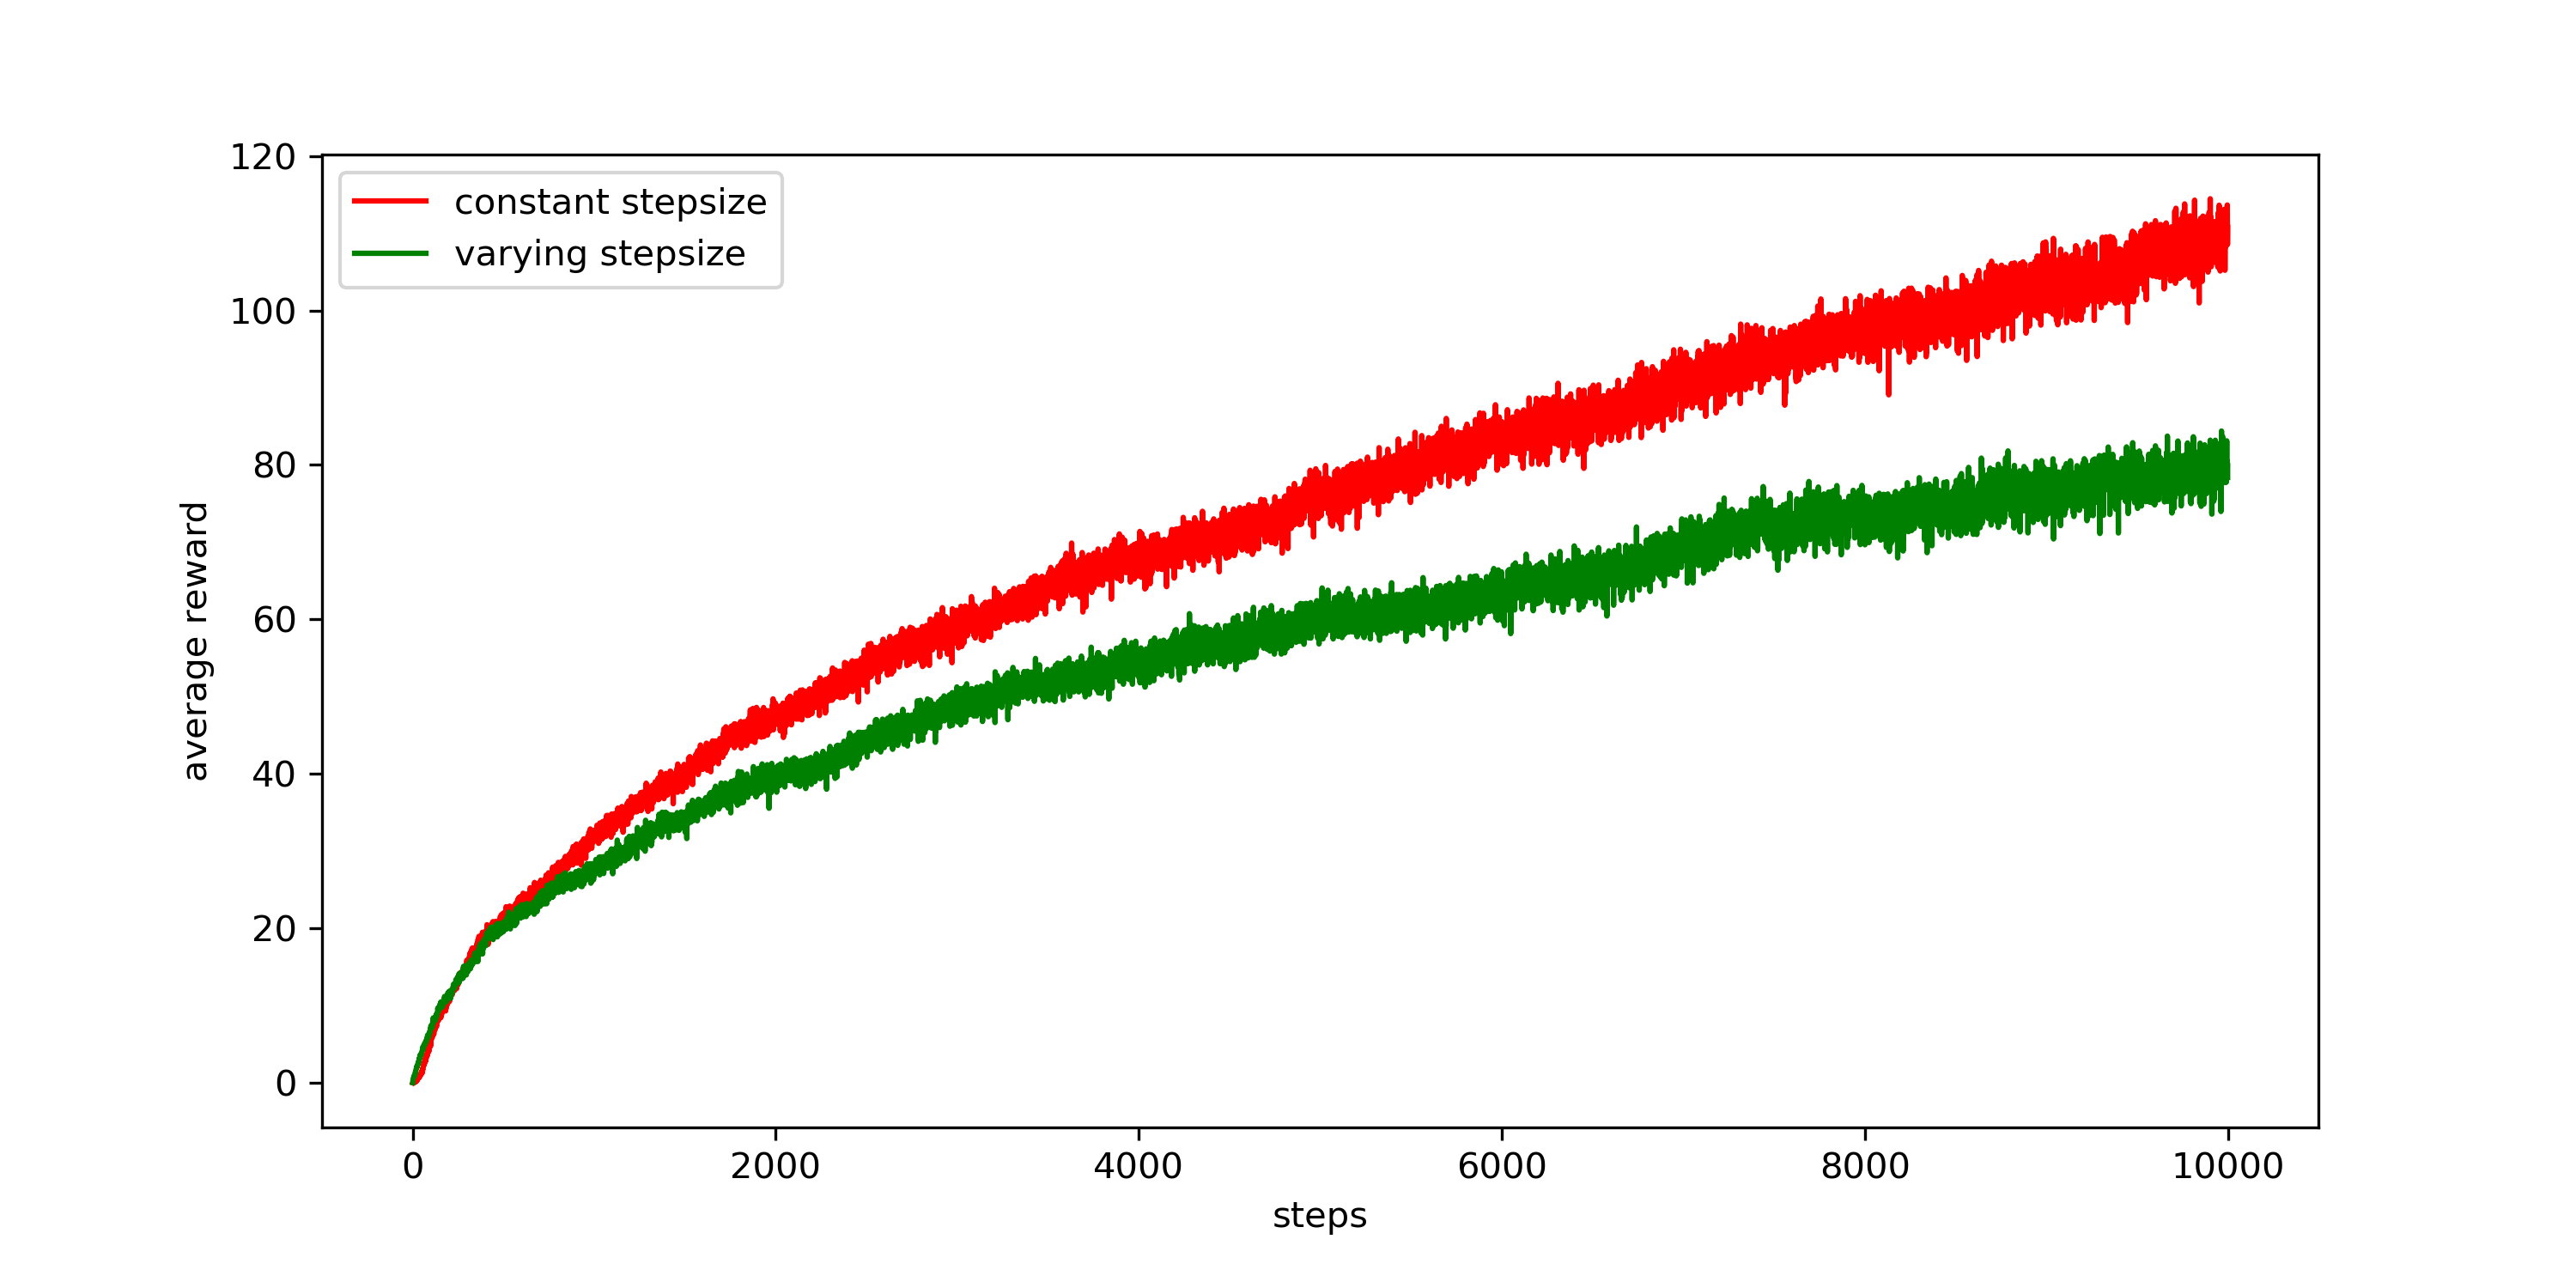
\includegraphics[width=\textwidth]{/ex2.5}
	\caption{Stationary versus varying stepsize \(alpha\) in a 10-armed bandit problem. We see that the constant stepsize parameter (exponential decay) performs better than the varying stepsize parameter as we place more weight on the recently observed (moving) values.}
	\label{fig:ex2.5}
\end{figure}
$
\hfill \blacksquare
$

\subsection{Exercise 2.6}
\begin{figure}[h!]
	\centering
	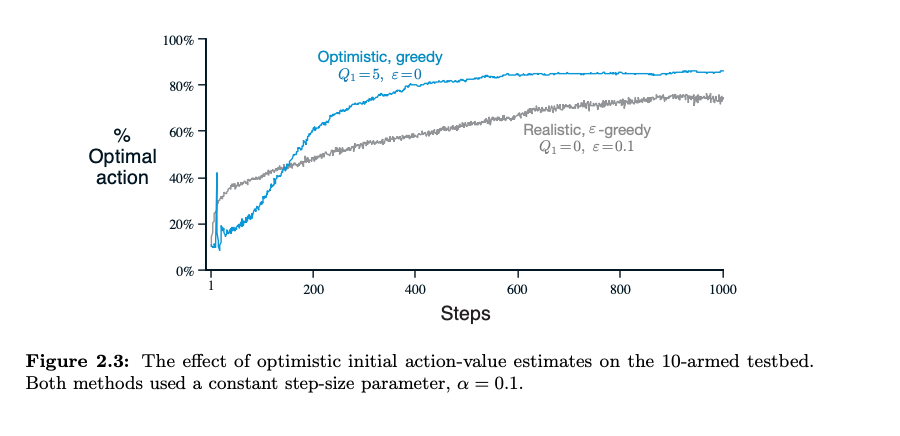
\includegraphics[width=\textwidth]{/chapter2_3}
	\caption{}
	\label{fig:chapter2_3}
\end{figure}

\subsubsection*{Q}
\textit{Mysterious Spikes}: The results shown in Figure 2.3 should be quite reliable because they are averages over 2000 individual, randomly chosen 10-armed bandit tasks. Why, then, are there oscillations and spikes in the early part of the curve for the optimistic
method? In other words, what might make this method perform particularly better or worse, on average, on particular early steps?

\subsubsection*{A}
The optimistic greedy policy with explore on every initial step as all value estimates are greater than their true value. It is possible, therefore, that it randomly selects the optimal action and then immediately forgets it in favour of yet-to-be-explored actions. This explains the spike at timestep \(\approx 10\).
$
\hfill \blacksquare
$

\subsection{Exercise 2.7}
\subsubsection*{Q}
Unbiased Constant-Step-Size Trick In most of this chapter we have used sample averages to estimate action values because sample averages do not produce the initial bias that constant step sizes do (see the analysis leading to (2.6)). However, sample averages are not a completely satisfactory solution because they may perform poorly on nonstationary problems. Is it possible to avoid the bias of constant step sizes while retaining their advantages on nonstationary problems? One way is to use a step size of
\begin{equation}
	\beta_n = \alpha / \bar{o_n}
\end{equation}

to process the \(n\)th reward for a particular action, where \(\alpha\) > 0 is a conventional constant step size, and ¯on is a trace of one that starts at 0:
\begin{equation}
	\bar{o_n} = \bar{o_{n-1}} + \alpha(1 - \bar{o_{n-1}}), for n > 0 and \bar{o_0} = 0.
\end{equation}

Carry out an analysis like that in (2.6) to show that Qn is an exponential recency-weighted
average without initial bias.

\subsubsection*{A}
If we recall our answer for Exercise 2.4 for varying stepsize, we see that \(Q_1\) is weighted by \(w = \prod_{i=1}^{\infty} (1 - \alpha_i)\). When \(i\) = 1, \(\beta_n\) = \(\alpha\), thus \(w \rightarrow 0 \forall i\) and \(Q_1\) no longer affects our estimate of \(Q_{n+1}\).
$
\hfill \blacksquare
$

\subsection{Exercise 2.8}
\subsubsection*{Q}
\textit{UCB Spikes} In Figure \ref{fig:chapter2_2} the UCB algorithm shows a distinct spike in performance on the 11th step. Why is this? Note that for your answer to be fully satisfactory it must explain both why the reward increases on the 11th step and why it decreases on the subsequent steps. Hint: If c = 1, then the spike is less prominent.

\subsubsection*{A}
After 10 timesteps the UCB algorithm has explored all 10 actions as, until they are selected, their upper confidence bound is infinite (as \(N_t(a)\) = 0) as so it guarenteed to be selected once in the first 10 actions. At this point the agent has one sample to assess the expected value of each arm and the same confidence/uncertainty in each action. With c < 0 it is likely to pick the action with highest return from first sample, which will likely give it an similarly large reward, creating the spike. Now, the upper confidence bound for that action will decrease and the agent will select another, less valuable action, causing the decrease in performance at the next timestep.
$
\hfill \blacksquare
$

\subsection{Exercise 2.9}
\subsubsection*{Q}
Show that in the case of two actions, the soft-max distribution is the same as that given by the logistic, or sigmoid, function often used in statistics and artificial neural networks.

\subsubsection*{A}
Soft-max distribution is defined as:
\begin{equation}
	Pr{A_t = a} \approx \frac{e^{H_t(a)}}{\sum_{b=1}^{k} e^{H_t(b)}} \approx \pi_t(a)
\end{equation}

For two actions \(1\) and \(2\) this becomes:

\begin{align}
	A_t  &= \frac{e^{H_t(1)}}{e^{H_t(1) + e^{H_t(2)}}}  \\
	&= \frac{e^{H_t(1)}}{e^{H_t(1)}}{(1 + \frac{e^{H_t(2)}}{e^{H_t(1)}}}  \\
	&= \frac{1}{e^{H_t(1)}(1 + e^{-x}}  \\
\end{align}
i.e. the sigmoid function with $x = H_t(1) - H_t(2)$.
$
\hfill \blacksquare
$

\subsection{Exercise 2.10}
\subsubsection*{Q}
Suppose you face a 2-armed bandit task whose true action values change randomly from time step to time step. Specifically, suppose that, for any time step, the true values of actions 1 and 2 are respectively 10 and 20 with probability 0.5 (case A), and 90 and 80 with probability 0.5 (case B). If you are not able to tell which case you face at any step, what is the best expected reward you can achieve and how should you behave to achieve it? Now suppose that on each step you are told whether you are facing case A or case B (although you still don’t know the true action values). This is an associative search task. What is the best expected reward you can achieve in this task, and how should you behave to achieve it?

\subsubsection*{A}
Part 1): If we do not know whether we are in task A or B we could decide pick the same action each time to maximise expected reward. Selecting either action 1 or action 2 every time would provide an expected reward of 50. Picking actions randomly would also provide an expected reward of 50 in this example.
Part 2): If we know we are in task A or B we can learn the optimal action for each (A(a) = 2 and B(a) = 1). Doing so would provide us a higher expected reward than the non-contextual case of 55.
$
\hfill \blacksquare
$
	\section{Finite Markov Decision Processes}
\subsection{Exercise 3.1}
\subsubsection*{Q}
Devise three example tasks of your own that fit into the MDP framework, identifying for each its states, actions, and rewards. Make the three examples as different from each other as possible. The framework is abstract and flexible and can be applied in many different ways. Stretch its limits in some way in at least one of your examples.

\subsubsection*{A}
\begin{enumerate}
	\item \textit{Golf: Putting}
	\begin{itemize}
		\item State: Coordinates of ball; coordinates of hole; x,y,z contour plot of green; grass length; grass type; wind speed; wind direction; ball type; putter type.
		\item Actions: (X, Y) direction of aim; length of stroke
		\item Rewards: -1 for each unit of distance from hole
	\end{itemize}
	\item \textit{Optimizing investment portfolio}
	\begin{itemize}
		\item State: Investment in each company; cash balance; \% return over last minute/hour/day/week/month/year
		\item Actions: For each investment: buy (discretized by some cash interval), sell (discretized by some cash interval), stick
		\item Rewards: +1 for each £ return per day 
	\end{itemize}
	\item \textit{Shoe-tying robot}
	\begin{itemize}
		\item State: Coordinates of laces; coordinates of robot arms/joints
		\item Actions: Grip pressure on laces; adjust position of arms to coordinates x,y,z
		\item Rewards: -1 for unit of shoe displacement from foot once tied.
	\end{itemize}
\end{enumerate}
$
\hfill \blacksquare
$
\subsection{Exercise 3.2}
\subsubsection*{Q}
Is the MDP framework adequate to usefully represent all goal-directed learning tasks? Can you think of any clear exceptions? 

\subsubsection*{A}
The MDP framework fails when the state cannot be fully observed. For example, one may try to control the temperature of a house using a state space represented by one thermometer in one room. Our agent would control the temperature observed by that thermometer well, but would be blind to temperatures that aren't measured by said thermometer elsewhere in the house.
$
\hfill \blacksquare
$

\subsection{Exercise 3.3}
\subsubsection*{Q}
Consider the problem of driving. You could define the actions in terms of the accelerator, steering wheel, and brake, that is, where your body meets the machine. Or you could define them farther out—say, where the rubber meets the road, considering your actions to be tire torques. Or you could define them farther in—say, where your brain meets your body, the actions being muscle twitches to control your limbs. Or you could go to a really high level and say that your actions are your choices of where to drive. What is the right level, the right place to draw the line between agent and environment? On what basis is one location of the line to be preferred over another? Is there any fundamental reason for preferring one location over another, or is it a free choice?

\subsubsection*{A}
There's a trade-off between state-action space complexity, computational expense and accuracy. If we draw the boundary at the brain we would create a state-action space contingent on the number of neurons in the brain and their interplay with physical actions like turning the steering wheel; too large to be stored or computed efficiently. Equally, if we draw the boundary at the \textit{journey} level, then we miss the detail required to act on second-by-second state changes on the road that could lead to a crash. The fundamental limiting factor in this selection is whether the goal can be achieved safely at your chosen layer of abstraction, indeed this feels like one of the tasks of engineering more widely.
$
\hfill \blacksquare
$

\subsection{Exercise 3.4}
\subsubsection*{Q}
Give a table analogous to that in Example 3.3, but for \(p(s0, r|s, a)\). It should have columns for \(s, a, s', r,\) and \(p(s0, r|s, a)\), and a row for every 4-tuple for which \(p(s0, r|s, a) > 0\).

\subsubsection*{A}
\begin{table}[]
	\begin{tabular}{llll|l}
\(s\) & \(a\) & \(s'\) & \(r\) & p(\(s, r, | s, a\)) \\ \hline 
$\mathnormal{high}$		& $ \mathnormal{search}$     & $\mathnormal{high} $       & \(r_{\mathnormal{search}}\)       &   \(\alpha\) \\
$\mathnormal{high}$		&  $\mathnormal{search}$     &  $\mathnormal{low}$      &   \(r_{\mathnormal{search}}\)     &  \((1-\alpha)\) \\                  
$\mathnormal{low}$		&  $\mathnormal{search}$     & $\mathnormal{high}$       & -3      & \((1-\beta)\)                    \\
$\mathnormal{low}$		&  $\mathnormal{search}$    & $\mathnormal{low} $       &  \(r_{\mathnormal{search}}\)      & \(\beta\) \\                     
$\mathnormal{high}$		&  $\mathnormal{wait}$     & $\mathnormal{high}$       & \(r_{\mathnormal{wait}}\)       &   1   \\
$\mathnormal{low}$		&  $\mathnormal{wait}$   & $\mathnormal{low}$       &  \(r_{\mathnormal{wait}}\)      &  1  \\
$\mathnormal{low}$		&  $\mathnormal{recharge}$   & $\mathnormal{high}$       &  0      &   1       \\
	\end{tabular}
\end{table}

As there is no probability distribution over the rewards (i.e. for each state-action pair, the agent receives some reward with \(p(r) = 1\))), \(p(s', r | s, a) = p(s' | s, a)\).
$
\hfill \blacksquare
$

\subsection{Exercise 3.5}
\subsubsection*{Q}
The equations in Section 3.1 are for the continuing case and need to be modified (very slightly) to apply to episodic tasks. Show that you know the modifications needed by giving the modified version of (3.3). 

\subsubsection*{A}
Equation 3.3 from section 3.1 is:

\begin{equation}
	\sum_{s' \in S} \sum_{r \in R} p(s', r | s, a) = 1, \forall s \in S, a \in A(s)
\end{equation}

for episodic tasks this becomes:

\begin{equation}
\sum_{s' \in S^+} \sum_{r \in R} p(s', r | s, a) = 1, \forall s \in S, a \in A(s)
\end{equation}
$
\hfill \blacksquare
$

\subsection{Exercise 3.6}
\subsubsection*{Q}
Suppose you treated pole-balancing as an episodic task but also used discounting, with all rewards zero except for 1 upon failure. What then would the return be at each time? How does this return differ from that in the discounted, continuing formulation of this task? 

\subsubsection*{A}
In the discounted, episodic version of the pole-balancing task, the return after each episode is:

\begin{equation}
	G_t = -\gamma^{T-t}
\end{equation}

where \(T\) is the timestep at which the episode ends i.e. the task is failed. In the continuining case the cumulative return is:

\begin{equation}
G_t = -\sum_{K\in\mathcal{K}} \gamma^{K-1}
\end{equation}

where \(\mathcal{K}\) is the set of times where the task is failed. Note this reward will increase in the long run, irrespective of improved performance. Designing this as a continuous task does not therefore make sense here.
$
\hfill \blacksquare
$

\subsection{Exercise 3.7}
\subsubsection*{Q}
Imagine that you are designing a robot to run a maze. You decide to give it a reward of +1 for escaping from the maze and a reward of zero at all other times. The task seems to break down naturally into episodes—the successive runs through the maze—so you decide to treat it as an episodic task, where the goal is to maximize expected total reward (3.7). After running the learning agent for a while, you find that it is showing no improvement in escaping from the maze. What is going  wrong? Have you effectively communicated to the agent what you want it to achieve?

\subsubsection*{A}
We have designed the reward such that it receives +1 only once it has exited the maze, and are therefore not incentivising it to learn how to exit the maze faster. To do so, we would need to provide a negative reward proportional to time in the maze e.g. -1 per timestep.
$
\hfill \blacksquare
$

\subsection{Exercise 3.8}
\subsubsection*{Q}
Suppose \(\gamma\) = 0.5 and the following sequence of rewards is received R1 = -1, R2 = 2, R3 = 6, R4 = 3, and R5 = 2, with T = 5. What are \(G_0, G_1, \ldots, G_5\)? Hint: Work backwards.

\subsubsection*{A}
We know:
$
G_t = R_{t+1} + \gamma G_{t+1}
$
Therefore, for the terminal state:
$
G_5 = 0
$
then:
$
G_4 = 2 +  (0.5 \times 0) = 2
G_3 = 3 + (0.5 \times 2) = 4
G_2 = 6 + (0.5 \times 4) = 8
G_1 = 2 + (0.5 \times 8) = 6
G_0 = -1 + (0.5 \times 6) = 2
$
Note our expected cumulative reward \(G_t\) depends greatly on our instant reward \(G_{t+1}\) because it is not  discounted.
$
\hfill \blacksquare
$

\subsection{Exercise 3.9}
\subsubsection*{Q}
Suppose \(\gamma\)  = 0.9 and the reward sequence is $R_1$ = 2 followed by an infinite sequence of 7s. What are $G_1$ and $G_0?$

\subsubsection*{A}
We know that if the reward is an infinite series of 1s, $G_t$ is:
$
G_t = \sum_{k=0}^{\infty} \gamma^k = \frac{1}{1-\gamma}
$

So for an infinite series of 7s this becomes:
$
G_t = \sum_{k=0}^{\infty} \gamma^k = \frac{7}{0.1}
$
\\
Therefore:
\begin{align}
G_0 &= 2 + \frac{7}{0.1} \\
&= 72\\
\end{align}
and 
\begin{align}
G_1 &= 7 + \frac{7}{0.1} \\
&= 77\\
\end{align}
$
\hfill \blacksquare
$

\subsection{Exercise 3.10}
\subsubsection*{Q}
Prove the second equality in (3.10). 

\subsubsection*{A}
$
G_t = \sum_{k=0}^{\infty} \gamma^k
$
\\
Expanding out the geometric series we get:
\begin{align}
s &= a + a\gamma + a\gamma^2 + \ldots + a\gamma^n\\
s\gamma &= a\gamma + a\gamma^2 + a\gamma^3+ \ldots + a\gamma^{n+1}\\
\end{align}

Subtract the first series from the second series and we get:
\begin{align}
s -s\gamma &= a - a\gamma^{n+1} \\
s(1 - \gamma) &= a(1 - \gamma^{n+1}) \\
s &= \frac{a(1 - \gamma^{n+1})}{1 - \gamma} \\
\end{align}

If $|\gamma| < 0$,  in the limit as n $\rightarrow \infty$ we get:
\begin{equation}
s = \frac{a}{1 - \gamma}
\end{equation}

and in our special case $a = 0$ so:
\begin{equation}
s = G_t =  \frac{1}{1 - \gamma}
\end{equation}
$
\hfill \blacksquare
$

\subsection{Exercise 3.11}
\subsubsection*{Q}
If the current state is $S_t$, and actions are selected according to a stochastic policy \(\pi\), then what is the expectation of $R_{t+1}$ in terms of $\pi$ and the four-argument function \(p\) (3.2) 

\subsubsection*{A}
$
\mathbb{E}_\pi[R_{t+1} | s_t] = \sum_{a} \pi(a | s) \sum_{s'} \sum_{r} p(s', r | s, a) [r] 
$
$
\hfill \blacksquare
$

\subsection{Exercise 3.12}
\subsubsection*{Q}
Give an equation for $v_\pi$ in terms of $q_\pi$ and $\pi$. 

\subsubsection*{A}
The state value function \(v_\pi\) is equal to the expected cumulative return from that state given a distribution of actions. The state-action value function \(q_\pi\) is the value of being in a state and taking a deterministic action. Therefore the state value function is the weighted sum of the state action value function, with the weights equal to the probabilities of selecting each action:
$
v_\pi = \sum_{a} \pi(a | s) q_\pi(s,a) 
$
$
\hfill \blacksquare
$

\subsection{Exercise 3.13}
\subsubsection*{Q}
Give an equation for $q_\pi$ in terms of $v_\pi$ and the four-argument $p$.  

\subsubsection*{A}
Given an action $a$, the state-action value function is the probability distributions over the possible next states and rewards from that action, times the one-step reward and the discounted state value function at the next timestep:
$
q_\pi = \sum_{s' \in \mathcal{S}} \sum_{r \in \mathcal{R}} p(s', r | s, a) [r + \gamma v_\pi(s_{t+1})]
$
$
\hfill \blacksquare
$

\subsection{Exercise 3.14}
\begin{figure}[h!]
	\centering
	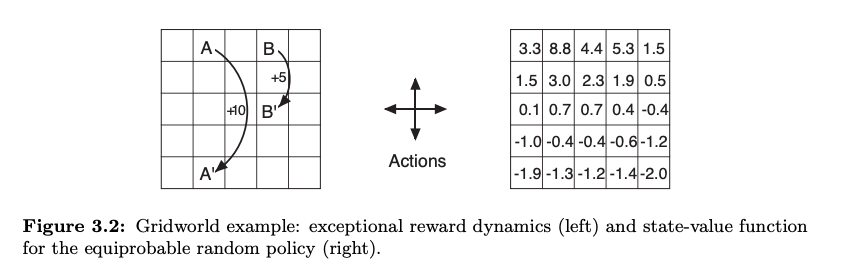
\includegraphics[width=\textwidth]{/ex3.14}
	\caption{Gridworld example for ex. 3.14}
	\label{fig:3.14}
\end{figure}

\subsubsection*{Q}
The Bellman equation (3.14) must hold for each state for the value function $v_\pi$ shown in Figure 3.2 (right) of Example 3.5. Show numerically that this equation holds for the center state, valued at +0.7, with respect to its four neighbouring states, valued at +2.3, +0.4, 0.4, and +0.7. (These numbers are accurate only to one decimal place.) .  

\subsubsection*{A}
Bellman equation for $v_\pi$ is:
\begin{equation}
v_\pi(s) = \sum_{a} \pi(a | s) \sum_{s', r} p(s', r | s, a) [r + \gamma v_\pi(s')] 
\end{equation}
for the centre square in Figure \ref{fig:3.14} we get the following:
\begin{align}
v_\pi(s) &= 0.25 \left[0.9 \times 2.3\right] + 0.25 \left[0.9 \times 0.7\right] + 0.25 \left[0.9 \times 0.4\right] + 0.25 \left[0.9 \times -0.4\right] \\
			&= 0.68 \approx 0.7 \\
\end{align}
$
\hfill \blacksquare
$

\subsection{Exercise 3.15}
\subsubsection*{Q}
In the gridworld example, rewards are positive for goals, negative for running into the edge of the world, and zero the rest of the time. Are the signs of these rewards important, or only the intervals between them? Prove, using (3.8), that adding a constant $c$ to all the rewards adds a constant, $v_c$, to the values of all states, and thus does not affect the relative values of any states under any policies. What is $v_c$ in terms of $c$ and $\gamma$? 

\subsubsection*{A}
Part 1): The sign of the reward is of no consequence, it is indeed the interval between each reward that drives behaviour.
Part 2): Equation 3.8 is as follows:
\begin{equation}
G_t = \sum_{k=0}^{\infty} \gamma^k R_{t+k+1}
\end{equation}
when we add a constant $c$ to all rewards this becomes:
$
G_t = \sum_{k=0}^{\infty} \gamma^k [R_{t+k+1} + c]
G_t = \frac{R_{t+k+1}}{1 - \gamma} + \frac{c}{1 - \gamma}
$

Expected cumulative reward from every state receives a constant additive term. \(v_c\) in terms of $c$ and $\gamma$ is:
\begin{align}
v_c &= \mathbb{E}\left[\sum_{k=0}^{\infty}\gamma^k c\right]\\
&= \frac{c}{1 - \gamma}\\
\end{align}
$
\hfill \blacksquare
$

\subsection{Exercise 3.16}
\subsubsection*{Q}
Now consider adding a constant $c$ to all the rewards in an episodic task, such as maze running. Would this have any effect, or would it leave the task unchanged as in the continuing task above? Why or why not? Give an example. 

\subsubsection*{A}
In the episodic task adding a constant to all rewards does affect the agent. Since the cumulative reward now depends on the length of the episode ($G_t = \sum_{k=t+1}^{T} \gamma^{k-t-1}R_k $), timesteps that incur positive rewards act to lengthen the episode and vice versa. In the maze running example, we may have chosen to give the agent -1 reward at each timestep to ensure it completes the task quickly. If we add $c=2$ to every reward such that the reward at each timestep is now positive, the agent is now incentivised to not find the exit, and continue collecting intermediate rewards indefinitely. 
$
\hfill \blacksquare
$

\subsection{Exercise 3.17}
\begin{figure}[h!]
	\centering
	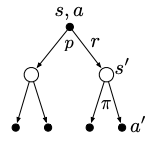
\includegraphics[width=0.25\textwidth]{/ex3.17}
	\caption{Backup diagram for $q_\pi$}
	\label{fig:3.17}
\end{figure}
\subsubsection*{Q}
What is the Bellman equation for action values, that is, for $q_\pi$? It must give the action value $q_\pi(s, a)$ in terms of the action values, $q_\pi(s0, a0)$, of possible successors to the state–action pair $(s, a)$. Hint: The backup diagram to the right corresponds to this equation. Show the sequence of equations analogous to (3.14), but for action values.

\subsubsection*{A}
\begin{align}
q_\pi(s,a) &= \mathbb{E}_\pi[G_t | S_t = s, A_t = a] \\
&= \mathbb{E}_\pi[R_{t+1} + \gamma G_{t+1} | S_t = s, A_t = a] \\
&= \sum_{s', r} p(s', r | s, a) [r + \gamma \mathbb{E}_\pi[G_{t+1} | s', a']] \\
&= \sum_{s', r} p(s', r | s, a) [r + \gamma q_\pi(s', a')] \\
\end{align}
$
\hfill \blacksquare
$

\subsection{Exercise 3.18}
\subsubsection*{Q}
\begin{figure}[h!]
	\centering
	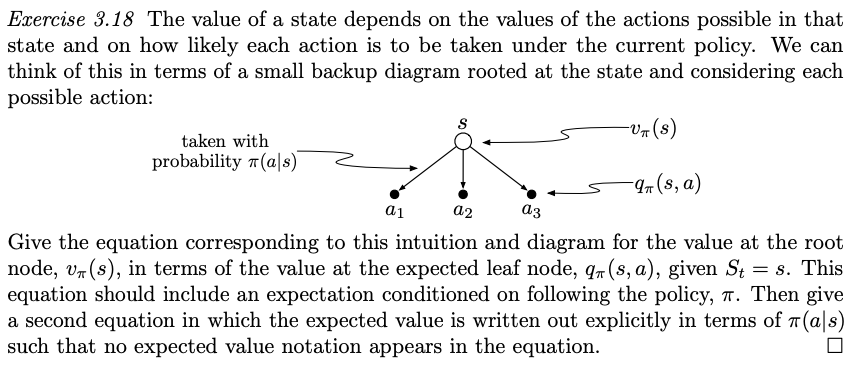
\includegraphics[width=\textwidth]{/ex3.18}
	\label{fig:3.18}
\end{figure}

\subsubsection*{A}
\begin{equation}
v_\pi(s) = \mathbb{E}_\pi \left[q_\pi(s,a)\right] 
v_\pi(s) = \sum_{a} \pi(a|s) q_\pi(s,a)
\end{equation}
$
\hfill \blacksquare
$

\subsection{Exercise 3.19}
\subsubsection*{Q}
\begin{figure}[h!]
	\centering
	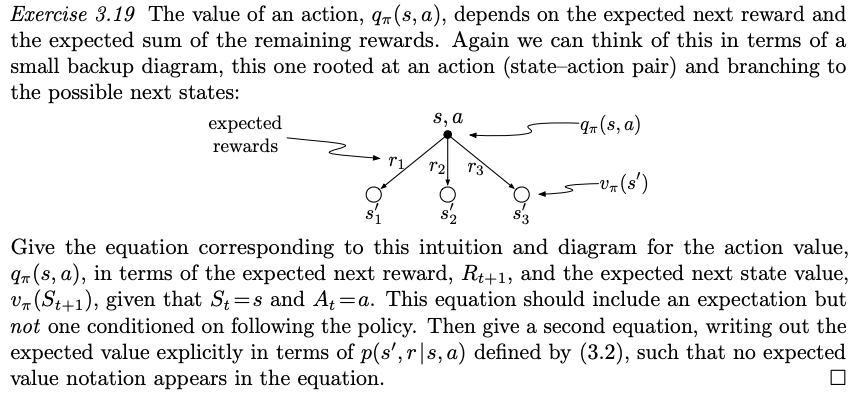
\includegraphics[width=\textwidth]{/ex3.19}
	\label{fig:3.19}
\end{figure}

\subsubsection*{A}
\begin{align}
q_\pi(s, a) &= \mathbb{E} \left[R_{t+1} + v_\pi(s') | S_{t} = s)\right] \\
&= \sum_{s', r} p(s', r | s, a) [r +v_\pi(s')] \\
\end{align}
$
\hfill \blacksquare
$

\subsection{Exercise 3.20}
\subsubsection*{Q}
\begin{figure}[h!]
	\centering
	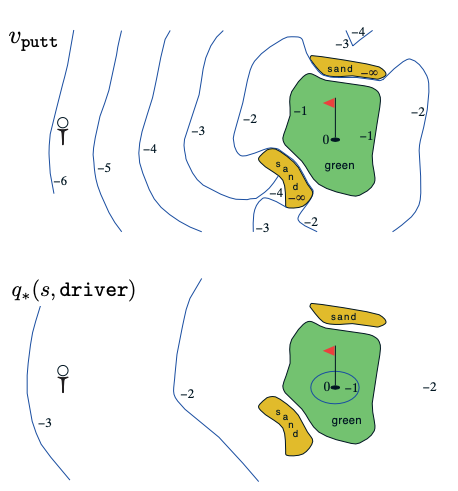
\includegraphics[width=0.5\textwidth]{/ex3.20}
	\caption{Value functions for golf.}
	\label{fig:3.20}
\end{figure}
Draw or describe the optimal state-value function for the golf example.

\subsubsection*{A}
Qualitatively, the optimal state-value function for golf (outlined by Figure \ref{fig:3.20}) would be derived from a policy that selected the driver for the first two shots (off-the green), then selected the putter for the final shot (on the green).
$
\hfill \blacksquare
$

\subsection{Exercise 3.21}
\subsubsection*{Q}
Draw or describe the contours of the optimal action-value function for putting, $q_*(s, \mathnormal{putter})$, for the golf example.

\subsubsection*{A}
The optimal action-value function is given by the following:
\begin{equation}
q_*(s,a)= \sum_{s', r} p(s', r | s, a) [r + \gamma \argmax_a q_*(s,a)]
\end{equation}

Since we have only one action($\mathnormal{putter}$), the argmax collapses to $v_*(s')$, and $q_*(s,a) = v_*(s)$ - illustrated in Figure \ref{fig:3.20}.
$
\hfill \blacksquare
$

\subsection{Exercise 3.22}
\subsubsection*{Q}
\begin{figure}[h!]
	\centering
	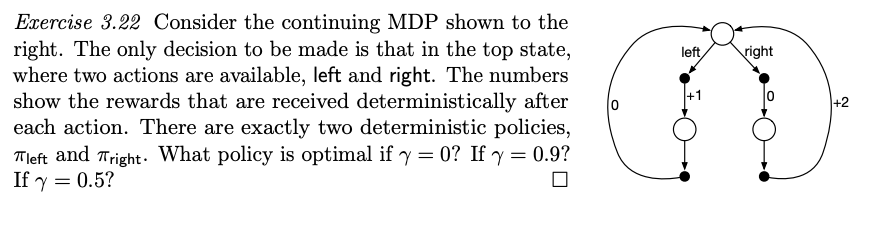
\includegraphics[width=\textwidth]{/ex3.22}
	\label{fig:3.20}
\end{figure}

\subsubsection*{A}
Let's first evaluate the simplest case of $\gamma = 0$. Recall that:
\begin{equation}
v_\pi(s) = \mathbb{E}_\pi[R_{t+1} + \gamma G_{t+1} | S_t = s]
\end{equation}

For $\pi_{left}$ we get:
\begin{align}
v_{\pi_{left}} &= 1 + \mathbb{E}_{\pi_{left}} \left[0 \times \gamma G_{t+1} \right] \\
v_{\pi_{left}} &= 1 \\
\end{align}

And for $\pi_{right}$ we get:
\begin{align}
v_{\pi_{left}} &= 0 + \mathbb{E}_{\pi_{left}} \left[0 \times \gamma G_{t+1} \right] \\
v_{\pi_{left}} &= 0 \\\
\end{align}

So the optimal policy for $\gamma = 0$ is $v_{\pi_{left}}$. If instead $\gamma = 0.9$, we get for $\pi_{left}$:

\begin{align}
v_{\pi_{left}} &= 1 + \mathbb{E}_{\pi_{left}} \left[0.9 \times G_{t+1} \right] \\
v_{\pi_{left}} &= 1 + \mathbb{E}_{\pi_{left}} \left[0.9 \times [r_{t+1} + \gamma G_{t+2}] \right],  \\
\end{align}

where $G_{t+2}$ is our expected reward back at our current state. We can negate it and just look at the first loop, as max reward over first loop will create max reward in the limit. Therefore:

\begin{align}
v_{\pi_{left}} &= 1 + 0.9 \times 0 = 1,\\
v_{\pi_{right}} &= 0 + 0.9 \times 2 = 1.8  \\
\end{align}

So the optimal policy for $\gamma = 0$ is $v_{\pi_{right}}$. If, finally, $\gamma = 0.5$, we get:
\begin{align}
v_{\pi_{left}} &= 1 + 0.5 \times 0 = 1,\\
v_{\pi_{right}} &= 0 + 0.5 \times 2 = 1  \\
\end{align}

So both polices are optimal.
$
\hfill \blacksquare
$

\subsection{Exercise 3.23}
\subsubsection*{Q}
Give the Bellman equation for $q_*$ for the recycling robot.

\subsubsection*{A}
$
q_*(s,a) =  \sum_{s',r} p(s',r | s, a) [r + \gamma \argmax_{a \in \mathcal{A}} q_*(s', a')]
$
where $\mathcal{A} = \{\mathnormal{search}, \mathnormal{wait}, \mathnormal{recharge}\}$
$
\hfill \blacksquare
$

\subsection{Exercise 3.24}
\subsubsection*{Q}
Figure 3.5 gives the optimal value of the best state of the gridworld as 24.4, to one decimal place. Use your knowledge of the optimal policy and (3.8) to express this value symbolically, and then to compute it to three decimal places.

\subsubsection*{A}
We can observe from the grid that $\gamma = 22/24.4 = 0.9016$

Equation 3.8 was:
\begin{equation}
G_t = R_{t+1} + \gamma R_{t+2} + \gamma^2 R_{t+3} + \gamma^3 R_{t+4} + \gamma^4 R_{t+5} + \gamma^5 R_{t+6} + \ldots =  \sum_{k=0}^{\infty} \gamma^k R_{t+k+1}
\end{equation}

We can represent the optimal value function $v_*$ as:
\begin{align}
v_*(A) &= r + \gamma(v_*(A+1)) \\
 &= 10 + 0.9016(16) \\
 &= 24.426 \text{to 3 d.p.} \\
\end{align}
$
\hfill \blacksquare
$

\subsection{Exercise 3.25}
\subsubsection*{Q}
Give an equation for $v_*$ in terms of $q_*$.

\subsubsection*{A}
$
v_*(s) = \max_{a \in \mathcal{A}} q_{\pi_*}(s,a)
$

i.e. returning to the diagram in exercise 3.18, $v_*$ is defined as selecting the action (in that case of a possible 3) that produces the highest state-action value function
$
\hfill \blacksquare
$

\subsection{Exercise 3.26}
\subsubsection*{Q}
Give an equation for $q_*$ in terms of $v_*$ and the four-argument $p$.

\subsubsection*{A}
$
q_*(s,a) = \max \sum_{s', r} p(s', r | s, a)[r + v_*(s)]
$
$
\hfill \blacksquare
$

\subsection{Exercise 3.27}
\subsubsection*{Q}
Give an equation for $\pi_*$ in terms of $q_*$

\subsubsection*{A}
The optimal policy is the one that acts greedily w.r.t the optimal state-action value function i.e. it picks the action that has the highest $q(s,a)$ in the following state.
$
\pi_*(a|s) = \max_{a \in \mathcal{A}(s)} q_*(s',a)
$
$
\hfill \blacksquare
$

\subsection{Exercise 3.28}
\subsubsection*{Q}
Give an equation for $\pi_*$ in terms of $v_*$ and the four-argument $p$.

The optimal policy is the one that acts greedily w.r.t the optimal state value function conditioned on the system dynamics
\subsubsection*{A}
$
\pi_*(a|s) = \max_{a \in \mathcal{A}(s)} \sum_{s', r} p(s', r | s, a)[r  v_*(s')]
$
$
\hfill \blacksquare
$

\subsection{Exercise 3.29}
\subsubsection*{Q}
Rewrite the four Bellman equations for the four value functions ($v_\pi, v_*, q_\pi,and q_*$) in terms of the three argument function $p$ (3.4) and the two-argument function $r$ (3.5).

\subsubsection*{A}
tbc
$
\hfill \blacksquare
$
	\section{Dynamic Programming}

\subsection*{Exercise 4.1}
\subsubsection{Q}
In Example 4.1, if $\pi$ is the equiprobable random policy, what is $q_\pi(11, \mathnormal{down})$? What is $q_\pi(7, \mathnormal{down})$? 
\subsubsection{A}
The Bellman equation for $q(s,a)$ is:
\begin{equation}
q_\pi(s,a) = \sum_{s',r} p(s', r | s, a) \left[r + \gamma \sum_{a'} \pi(a' | s') q_\pi(s', a')\right]
\end{equation}

For the state-action pairs posed in the question, the Bellman equation becomes:
\begin{align}
q_\pi(11, \mathnormal{down}) &= -1 \\
q_\pi(7, \mathnormal{down}) &= -1 + -14 \\
&= -15 \\
\end{align}

as $\gamma = 1$ because MDP is undiscounted.

\subsection*{Exercise 4.2}
\subsubsection{Q}
In Example 4.1, suppose a new state 15 is added to the gridworld just below state 13, and its actions, \textit{left, up, right, and down}, take the agent to states 12, 13, 14, and 15, respectively. Assume that the transitions from the original states are unchanged. What, then, is $v_pi(15)$ for the equiprobable random policy? Now suppose the dynamics of state 13 are also changed, such that action $\mathnormal{down}$ from state 13 takes the agent to the new state 15. What is $v_\pi(15)$ for the equiprobable random policy in this case?
\subsubsection{A}
\begin{align}
v_\pi(15) &= 0.25 \left[(-1 + -20) + (-1 + -22) + (-1 + -14) + (-1 + v_\pi(15)) \right] \\
&= 0.25 \left[(-60 + v_\pi(15)) \right] \\
&= -15 + 0.25 \left[v_\pi(15) \right] \\
\end{align}

and we know $v_\pi(15) == v_\pi(13) == -20$ as the state transitions and value functions at next state are identical. Therefore we get:
\begin{align}
v_\pi(15) &= -15 + 0.25 \left[-20\right] \\
&= -20 \\
\end{align}

If the dynamics are changed such one can transition from state 13 into 15, the characteristic of the MDP are unchanged. Moving into state 15, which has the same value as state 13 and the same subsequent dynamics, is identical to returning back to state 13 - as was the case previously. The value function is therefore unchanged and $v_\pi(15) = -20$

\subsection*{Exercise 4.3}
\subsubsection{Q}
What are the equations analogous to (4.3), (4.4), and (4.5), but for action-value functions instead of state-value functions?
\subsubsection{A}
\begin{align}
q_\pi(s) &= \mathbb{E}_\pi \left[R_{t+1} + \gamma q_\pi(S_{t+1}, A_{t+1} | S_t = s, A_t = a)\right]v_\pi(s) \\
q_\pi(s,a) &= \sum_{s',r} p(s', r | s, a) \left[r + \gamma \sum_{a'} \pi(a' | s') q_\pi(s', a')\right] \\
q_{k+1}(s,a) &= \sum_{s',r} p(s', r | s, a) \left[r + \gamma \sum_{a'} \pi(a' | s') q_k(s', a')\right] \\
\end{align}

\subsection*{Exercise 4.4}
\subsubsection{Q}
The policy iteration algorithm on page 80 has a subtle bug in that it may never terminate if the policy continually switches between two or more policies that are equally good. This is okay for pedagogy, but not for actual use. Modify the pseudocode so that convergence is guaranteed.
\subsubsection{A}
When taking the argmax over $a$ in the policy improvement step of the algorithm, it's possible that we continue to flip backward and forward between two actions that are both optimal forever. At the moment, a tie is broken by randomly selecting between the value maximising actions. We could instead always select the first action to result from the argmax, this way we would ensure that the same optimal action is picked during iteration, switching the \textit{policy-stable} boolean to true, and ensuring convergence.

\subsection*{Exercise 4.5}
\subsubsection{Q}
How would policy iteration be defined for action values? Give a complete algorithm for computing $q_*$, analogous to that on page 80 for computing $v_*$. Please pay special attention to this exercise, because the ideas involved will be used throughout the rest of the book.
\subsubsection{A}
\begin{enumerate}
	\item \textbf{Initialization}: $q(s,a)$ and $\pi(s)$ initialised arbitrarily as before
	\item \textbf{Policy Evaluation}: Loop for each state-action pair $(s,a)$, $s \in \mathcal{S}, a \in \mathcal{A}$:\\
	\begin{equation}
	\begin{aligned}
		q \leftarrow Q(s,a) \\
		Q(s,a) \leftarrow \sum_{s',r} p(s', r | s, a) \left[r + \gamma \sum_{a'} \pi(a' | s') Q(s', a')\right] \\
		\delta \leftarrow max(\delta, |q - Q(s,a)|)
	\end{aligned}
	\end{equation}
	\item \textbf{Policy Improvement}: \\
	\begin{equation}
	\begin{aligned}
		\text{policy-stable} \leftarrow True \\
		\text{Loop for each state-action pair (s,a), s $\in \mathcal{S}, a \in \mathcal{A}$}:\\
		old-action \leftarrow \pi(s)\\
		\pi(s) \leftarrow \argmax_a \sum_{s',r} p(s', r | s, a) \left[r + \gamma \sum_{a'} \pi(a' | s') q_\pi(s', a')\right] \\
		\text{if old-action} \neq \pi(s), \text{then policy-stable} \leftarrow False \\
		\text{If policy-stable, then stop and return Q $\approx q_* and \pi \approx \pi_*$; else return to 2.} \\
	\end{aligned}
	\end{equation}
\end{enumerate}

\subsection*{Exercise 4.6}
\subsubsection{Q}
Suppose you are restricted to considering only policies that are $\epsilon$-soft, meaning that the probability of selecting each action in each state, $s$, is at least $\epsilon /|\mathcal{A}(s)|$. Describe qualitatively the changes that would be required in each of the steps 3, 2, and 1, in that order, of the policy iteration algorithm for $v_*$ on page 80.
\subsubsection{A}
During the policy improvement step (3), instead of the argmax creating a deterministic action in a state, we would update the policy such that each action $a \in \mathcal{A}$ would receive probability p(a) = $\epsilon /|\mathcal{A}(s)|$, then the max action would receive probability $1 - \epsilon + \epsilon /|\mathcal{A}(s)|$. The output policy is therefore stochastic, not deterministic. During the policy evaluation step (2), instead of looping over the states only, we would loop over all states and actions, weighting the value of each state-action by the probability of the action being selecting according to our $\epsilon$-soft policy. In step one, the policy would need to be initialised with an arbitrary distribution over the action space in each state.

\subsection*{Exercise 4.7}
\subsubsection{Q}
Write a program for policy iteration and re-solve Jack’s car rental problem with the following changes. One of Jack’s employees at the first location rides a bus home each night and lives near the second location. She is happy to shuttle one car to the second location for free. Each additional car still costs \$2, as do all cars moved in the other direction. In addition, Jack has limited parking space at each location. If more than 10 cars are kept overnight at a location (after any moving of cars), then an additional cost of \$4 must be incurred to use a second parking lot (independent of how many cars are kept there). These sorts of non-linearities and arbitrary dynamics often occur in real problems and cannot easily be handled by optimization methods other than dynamic programming. To check your program, first replicate the results given for the original problem.
\subsubsection{A}
\ProgrammingExercise

\subsection*{Exercise 4.8}
\subsubsection{Q} Why does the optimal policy for the gambler’s problem have such a curious form? In particular, for capital of 50 it bets it all on one flip, but for capital of 51 it does not. Why is this a good policy?
\subsubsection{A}
When the coin is bias against us it makes sense to minimise the number of flips we make as, in the limit, we cannot win. Consequently, we can win with probability 0.4 is we stake our full capital at 50. All other bets besides 50 are designed to get us back to 50 if we lose, or up to 50 if we win, from where we take our 40\% chance. For example, when our capital is 55, we stake 5, knowing that we are likely to fall back to 50 where we will go for the win.

\subsection*{Exercise 4.9}
\subsubsection{Q} Implement value iteration for the gambler’s problem and solve it for $p_h$ = 0.25 and $p_h$ = 0.55. In programming, you may find it convenient to introduce two dummy states corresponding to termination with capital of 0 and 100, giving them values of 0 and 1 respectively. Show your results graphically, as in Figure 4.3. Are your results stable as $\theta \rightarrow 0$?
\subsubsection{A}
\ProgrammingExercise

\begin{figure}[h!]
	\centering
	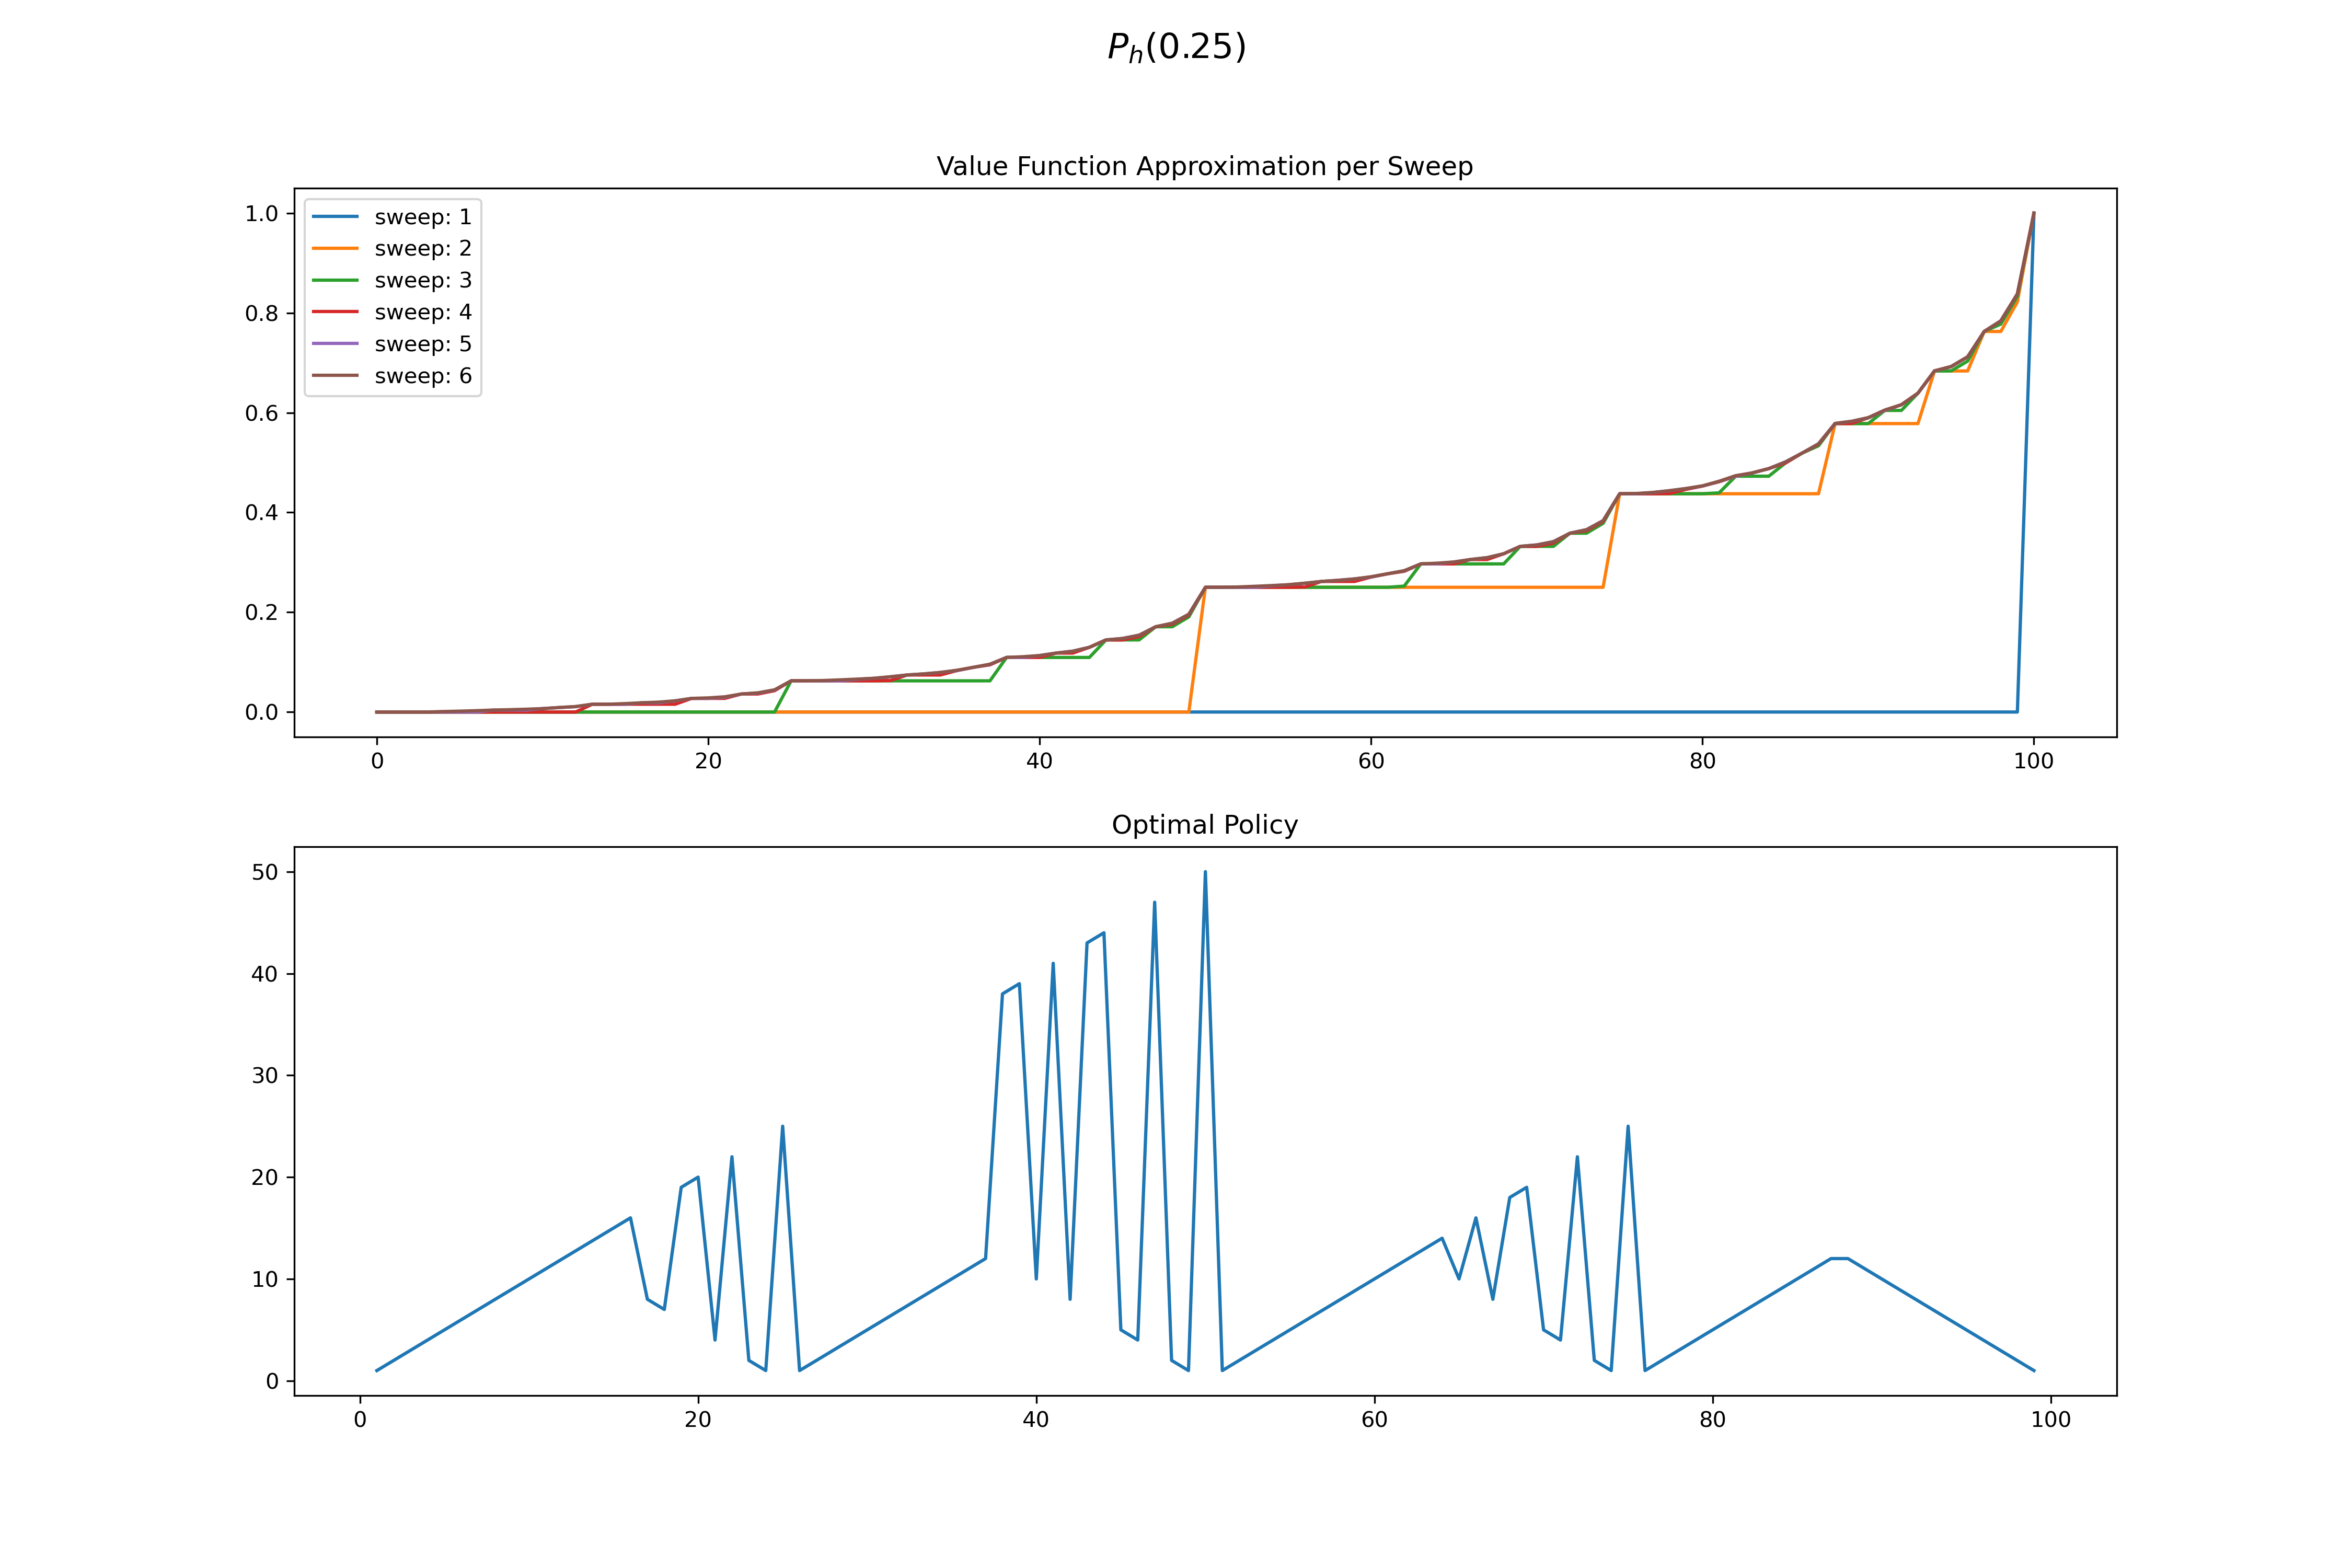
\includegraphics[width=\textwidth]{/ex4.9a}
	\label{fig:4.9a}
\end{figure}

\begin{figure}[h!]
	\centering
	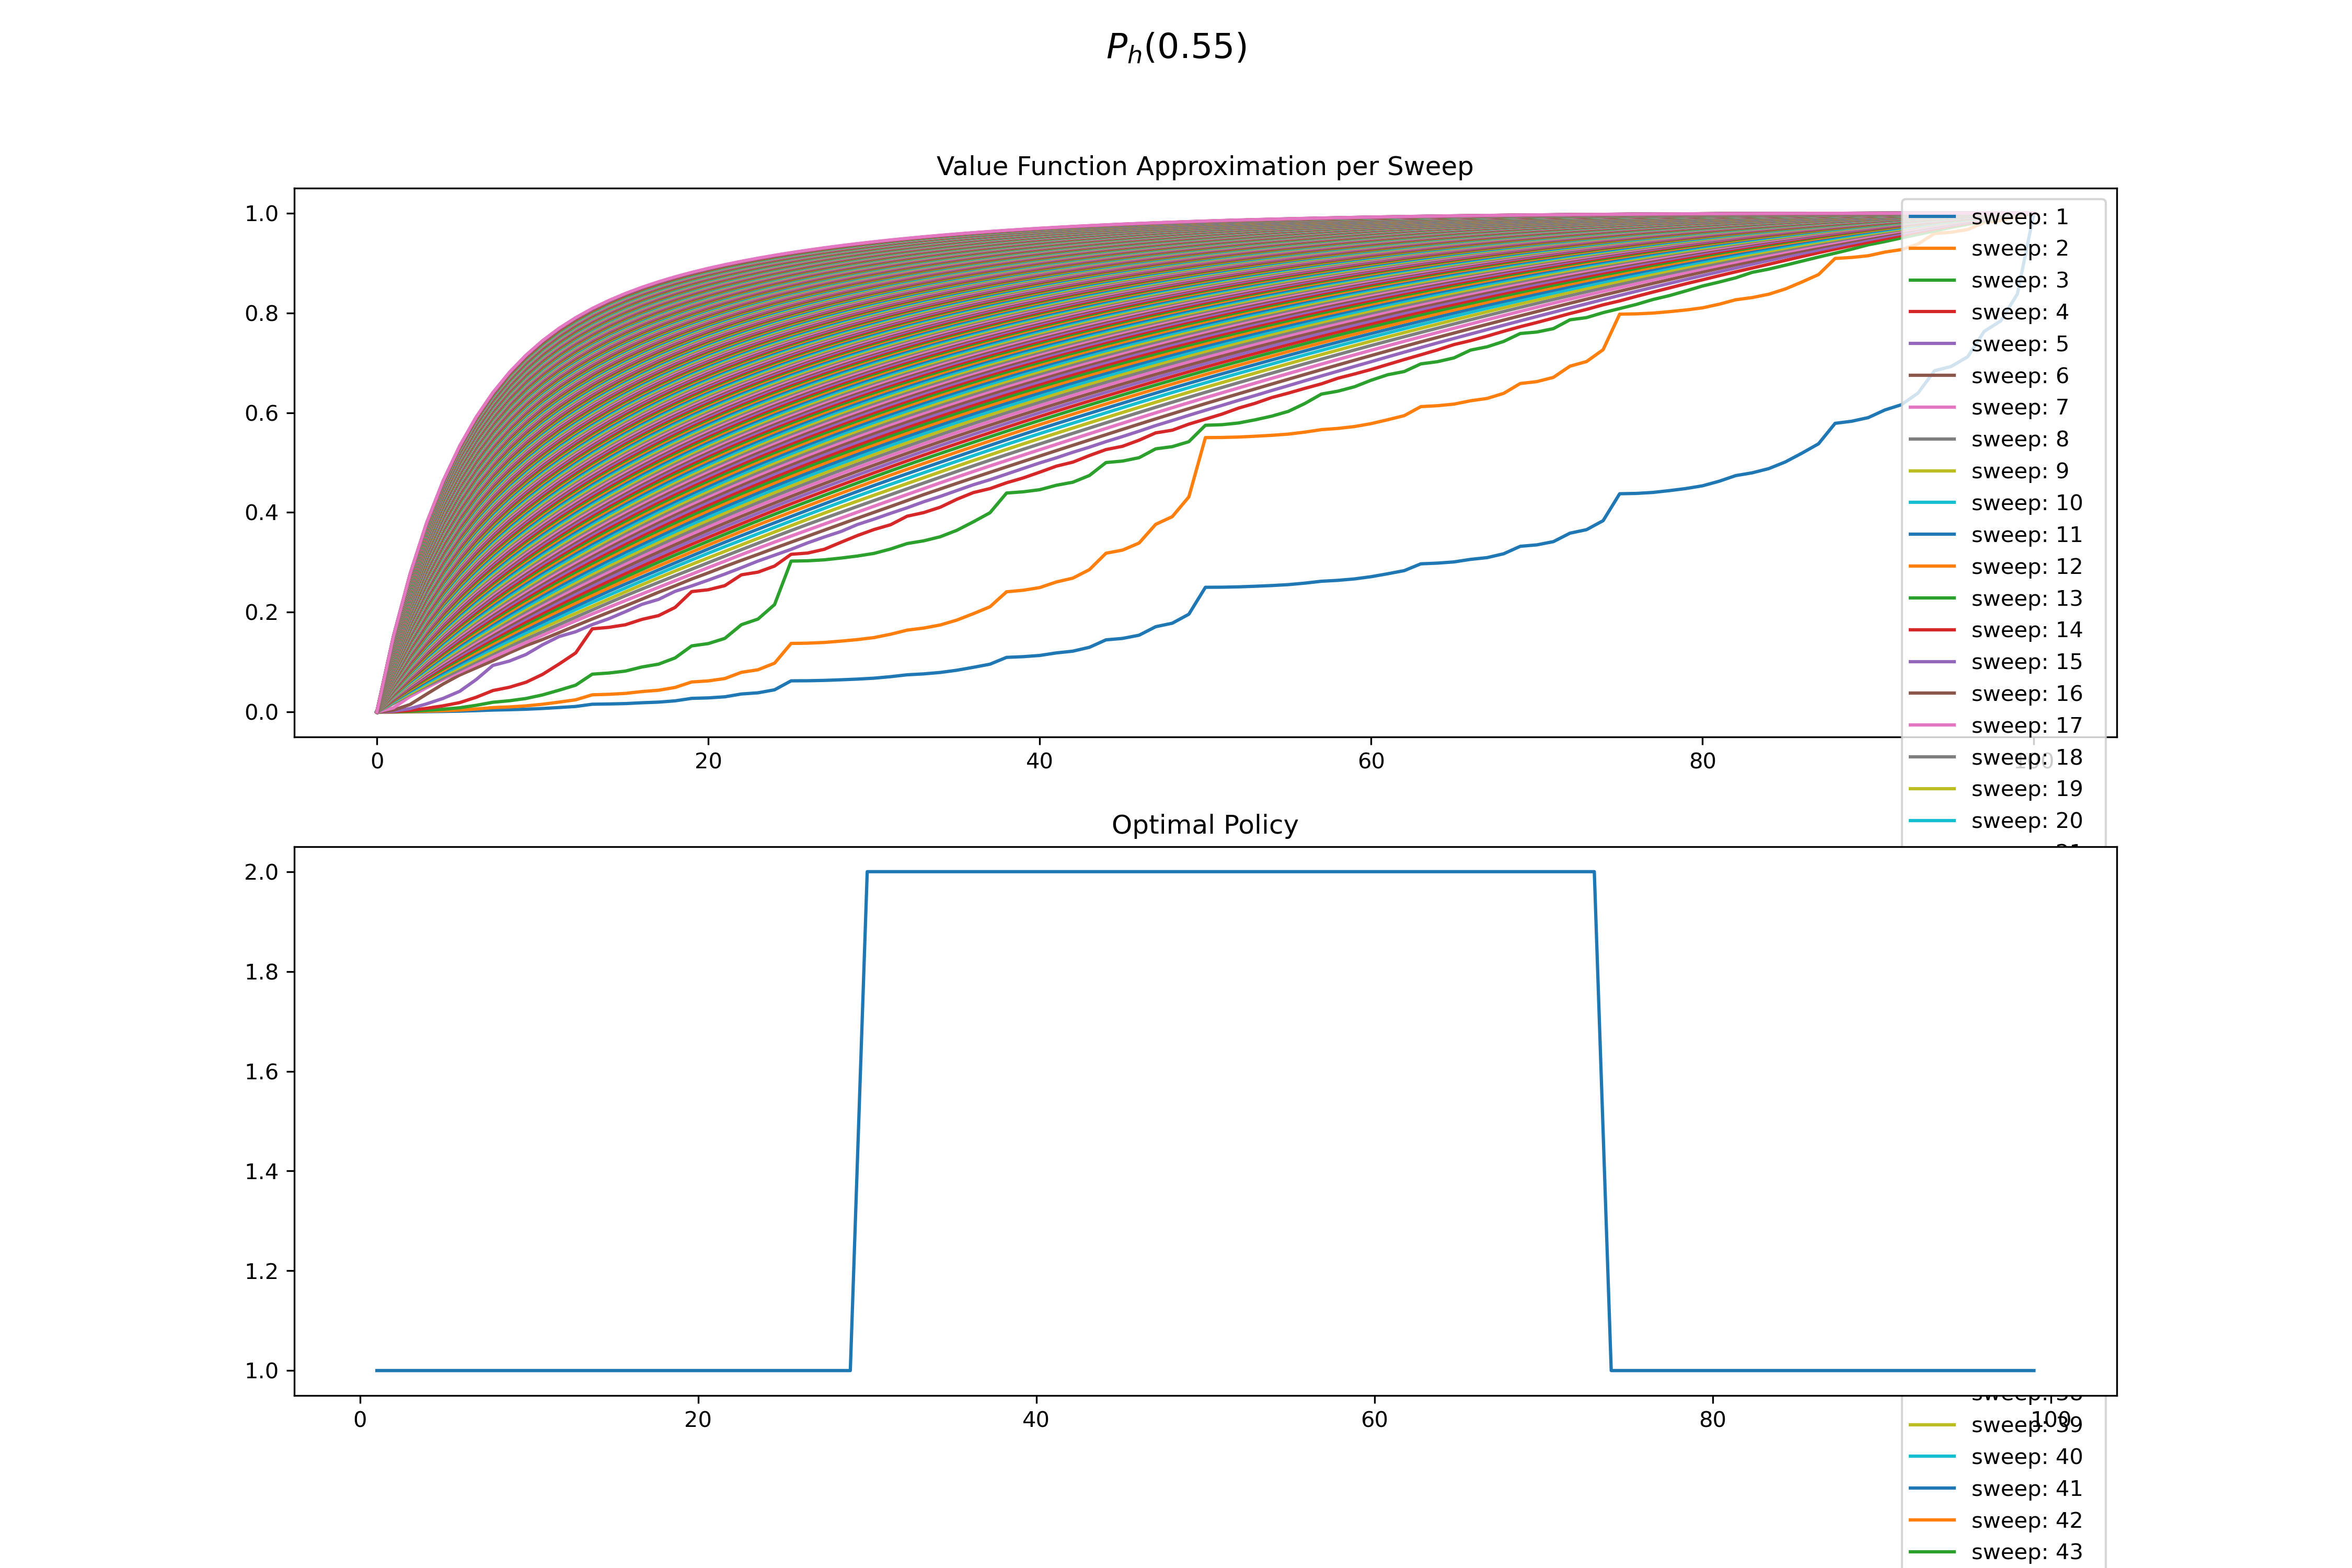
\includegraphics[width=\textwidth]{/ex4.9b}
	\label{fig:4.9b}
\end{figure}

\subsection*{Exercise 4.10}
\subsubsection{Q} What is the analog of the value iteration update (4.10) for action values, $q_{k+1}(s, a)$?
\subsubsection{A}
\begin{equation}
v_{k+1}(s) =  \sum_{s',r} p(s', r |s, a)\left[r + \gamma \argmax_{a'} q_k(s', a')\right]
\end{equation}

	\section{Monte Carlo Methods}

\subsection{Exercise 5.1}
\subsubsection{Q}
Consider the diagrams on the right in Figure 5.1. Why does the estimated value function jump up for the last two rows in the rear? Why does it drop off for the whole last row on the left? Why are the frontmost values higher in the upper diagrams than in the lower?
\subsubsection{A}
\begin{enumerate}
	\item The value function jumps for the rows in the rear because the player sticks at 20 and 21, where it is unlikely the dealer beat him given her policy to twist for all hands lower than 17.
	\item The value drops when the dealer holds an ace because it can be used to equal either 11 or 1, a stronger position than any of the other hands the dealer could hold.
	\item When an ace is usable, the value function is higher because the player can change the value of his ace from 11 to 1 if she is about to go bust.
\end{enumerate}
$
\hfill \blacksquare
$

\subsection{Exercise 5.2}
\subsubsection{Q}
Suppose every-visit MC was used instead of first-visit MC on the blackjack task. Would you expect the results to be very different? Why or why not?
\subsubsection{A}
The state is blackjack is monotonically increasing and memoryless (sampled with replacement), thus you can never revisit an old state in an episode once it has been first visited. Using every visit MC in this case would have no effect on the value function.
$
\hfill \blacksquare
$

\subsection{Exercise 5.3}
\subsubsection{Q}
What is the backup diagram for Monte Carlo estimation of $q_\pi$?
\subsubsection{A}
\begin{figure}[h!]
	\centering
	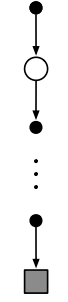
\includegraphics[width=0.05\textwidth]{/chapter5_2}
	\caption{Monte carlo backup diagram for estimation of $q_\pi$ from one episode}
	\label{fig:monte carlo qpi}
\end{figure}
$
\hfill \blacksquare
$

\subsection{Exercise 5.4}
\subsubsection{Q}
The pseudocode for Monte Carlo ES is inefficient because, for each state–action pair, it maintains a list of all returns and repeatedly calculates their mean. It would be more efficient to use techniques similar to those explained in Section 2.4 to maintain just the mean and a count (for each state–action pair) and update them incrementally. Describe how the pseudocode would be altered to achieve this.
\subsubsection{A}
Update formula from section 2.4 is:
\begin{equation}
	Q_n = Q_n + \frac{1}{n}\left[R_n - Q_n\right]
\end{equation}
As we reverse through the episode, we initialise value $N_{s,a}$ for each observed $s$ and $a$ to count the number of visits to the state. Instead of appending $G$ to returns, we use our now initialised $N$, and $G$ to update the value of $Q$. Doing so is more efficient as we don't need to hold a list of all returns which does not scale, we just update using the update rule outlined above.
$
\hfill \blacksquare
$

\subsection{Exercise 5.5}
\subsubsection{Q}
Consider an MDP with a single nonterminal state and a single action that transitions back to the nonterminal state with probability $p$ and transitions to the terminal state with probability $1 - p$. Let the reward be +1 on all transitions, and let $\gamma = 1$. Suppose you observe one episode that lasts 10 steps, with a return of 10. What are the first-visit and every-visit estimators of the value of the nonterminal state?
\subsubsection{A}
For first-visit estimator of the state is the return collected at the end of the episode having visited the first step, assuming we initialise $G=0$:
$
G = 10
$

The every-visit estimator is an average of each of the 10 returns received from the state:
\begin{equation}
G = \frac{1+2+3+4+5+6+7+8+9+10}{10} = 5.5
\end{equation}
$
\hfill \blacksquare
$

\subsection{Exercise 5.6}
\subsubsection{Q}
What is the equation analogous to (5.6) for action values $Q(s,a)$ instead of state values $V(s)$, again given returns generated using $b$?
\subsubsection{A}
Equation 5.6 is as follows:
\begin{equation}
V(s) = \frac{\sum_{t \in \mathcal{T}(s)} \rho_{t:T(t)-1} G_t}{\sum_{t \in \mathcal{T}(s)} \rho_{t:T(t)-1}}
\end{equation}

We only require that $\mathcal{T}$ tracks state action-pairs rather than just states. Equation 5.6 therefore becomes: 

\begin{equation}
Q(s,a) = \frac{\sum_{t \in \mathcal{T}(s,a)} \rho_{t:T(t)-1} G_t}{\sum_{t \in \mathcal{T}(s,a)} \rho_{t:T(t)-1}}
\end{equation}
$
\hfill \blacksquare
$

\subsection{Exercise 5.7}
\subsubsection{Q}
In learning curves such as those shown in Figure 5.3 error generally decreases with training, as indeed happened for the ordinary importance-sampling method. But for the weighted importance-sampling method error first increased and then decreased. Why do you think this happened?
\subsubsection{A}
In the initial episodes, we are unlikely to see episodes from the behaviour policy that match our target policy (i.e. hit for all card sums < 20 and stick thereafter), therefore our estimate for $V(s)$ will remain 0, which happens to be close to our ground truth $V_\pi(s)$. As we see some trajectories from $b$ that match our target policy, variance in our output will be high initially, leading to a higher error, and will drop gradually as we observe further trajectories until it approaches the true value asymptotically after 10,000 episodes.
$
\hfill \blacksquare
$

\subsection{Exercise 5.8}
\subsubsection{Q}
The results with Example 5.5 and shown in Figure 5.4 used a first-visit MC method. Suppose that instead an every-visit MC method was used on the same problem. Would the variance of the estimator still be infinite? Why or why not?
\subsubsection{A}
The variance of the estimator would remain infinite, as the expected return is still 1 for every-visit to the state. The only difference between first-visit and every-visit MC in this case is that the number of terms increases $\alpha$ to the number of visits to the state and so would continue to run to infinity.
$
\hfill \blacksquare
$

\subsection{Exercise 5.9}
\subsubsection{Q}
Modify the algorithm for first-visit MC policy evaluation (Section 5.1) to use the incremental implementation for sample averages described in Section 2.4. 
\subsubsection{A}
\begin{figure}[h!]
	\centering
	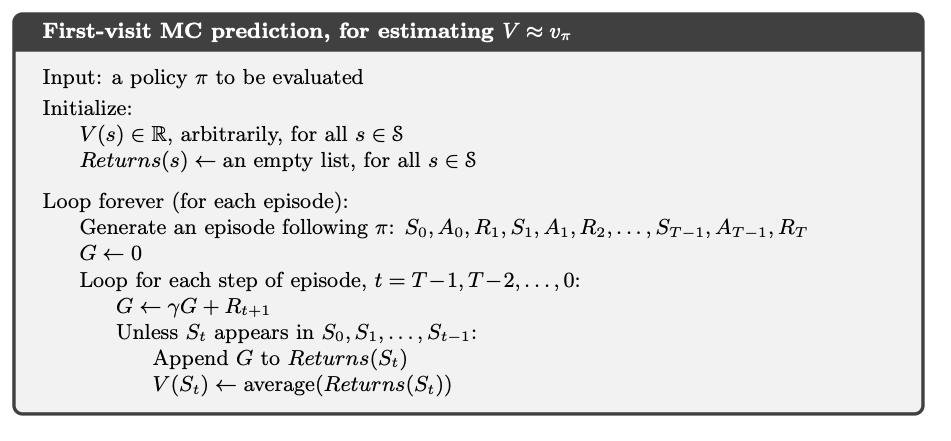
\includegraphics[width=0.75\textwidth]{/ex5.9}
	\label{fig:monte carlo policy eval}
\end{figure}

Modifying the above to include sample averages we change the last two lines. Instead of appending $G$ to $Returns(S_t)$ and averaging, we update $V(S_t)$ directly using:
$
V(S_t) = V(S_t) + \frac{1}{n}\left[G - V(S_t)\right]
$

to do this we need to initialise a new variable $n$ that counts the number of cross-episode visits to state $S_t$.
$
\hfill \blacksquare
$

\subsection{Exercise 5.10}
\subsubsection{Q}
Derive the weighted-average update rule (5.8) from (5.7). Follow the pattern of the derivation of the unweighted rule (2.3).
\subsubsection{A}
We have $C_o = 0$ and $C_n = \sum_{k=1}^{n} W_k$. Therefore:
\begin{align}
V_{n+1} &= \frac{\sum_{k=1}^{n}W_k G_k}{C_n}\\
V_{n+1}{C_n} &= \sum_{k=1}^{n}W_k G_k \\
V_{n+1}{C_n} &= W_n G_n \sum_{k=1}^{n-1}W_k G_k \\
V_{n+1}{C_n} &= W_n G_n + V_n \sum_{k=1}^{n-1}W_k \\
V_{n+1}{C_n} &= W_n G_n + V_n C_{n-1} \\
V_{n+1}{C_n} &= W_n G_n + V_n \left(C_n - W_n\right) \\
\vdots \\
V_{n+1} &= V_n + \frac{W_n}{C_n}\left[G_n - V_n\right] \\
\end{align}
$
\hfill \blacksquare
$

\subsection{Exercise 5.11}
\subsubsection{Q}
In the boxed algorithm for off-policy MC control, you may have been expecting the $W$ update to have involved the importance-sampling ratio $\frac{\pi (At|St)}{b(At|St)}$, but
instead it involves $\frac{1}{b(At|St)}$. Why is this nevertheless correct?
\subsubsection{A}
Because our policy $\pi(S_t)$ is a deterministic, greedy one, we are only observing trajectories where $\pi(A_t | S_t) = 1$, hence the numerator in the equation = 1.
$
\hfill \blacksquare
$

\subsection{Exercise 5.12}
\ProgrammingExercise
$
\hfill \blacksquare
$

\subsection{Exercise 5.13}
\subsubsection{Q}
Show the steps to derive (5.14) from (5.12). 
\subsubsection{A}
5.12 is:

\begin{align}
\rho_{t:T(t)-1} R_{t+1} &= R_{t+1} \prod_{k = t}^{T-1} \frac{\pi(A_k | S_k)}{b(A_k | S_k)} \\
\end{align}
$
\hfill \blacksquare
$

\subsection{Exercise 5.14}
\subsubsection{Q}
Modify the algorithm for off-policy Monte Carlo control (page 111) to use the idea of the truncated weighted-average estimator (5.10). Note that you will first need to convert this equation to action values.
\subsubsection{A}
...
$
\hfill \blacksquare
$
	\section{Temporal-Difference Learning}
\subsection{Exercise 6.1}
\subsubsection{Q}
If $V$ changes during the episode, then (6.6) only holds approximately; what would the difference be between the two sides? Let $V_t$ denote the array of state values
used at time $t$ in the TD error (6.5) and in the TD update (6.2). Redo the derivation above to determine the additional amount that must be added to the sum of TD errors in order to equal the Monte Carlo error.
\subsubsection{A}
Equation 6.5 becomes: $\delta_t = R_{t+1} + \gamma V_t(S_{t+1}) - V_t(S_t)$ and equation 6.2 becomes: $V_{t+1}(S_t) = V_t(S_t) + \alpha \left[R_{t+1} + \gamma V_t(S_{t+1} - V_t(S_t)\right]$. We then proceed as follows:
\begin{align}
G_t - V_t(S_t) &= R_{t+1} + \gamma G_{t+1} - V_t(S_t) + \gamma V_t(S_{t+1}) - \gamma V_t(S_{t+1}) \\
&= \delta_t + \gamma(G_{t+1} - V_t(S_{t+1})) \\
&= \delta_t + \gamma(G_{t+1} - V_{t+1}(S_{t+1})) + \gamma \theta_{t+1}, \text{with} \; \theta_{t} = \alpha \left[R_{t+1} + \gamma V_t(S_{t+1} - V_t(S_t))\right] \\
&= \delta_t + \gamma \delta_{t+1} + \gamma^2(G_{t+2} - V_{t+2}(S_{t+2})) + \gamma \theta_{t+1} + \gamma^2 \theta_{t+2} \\
&= \sum_{k=t}^{T-1} \left[\gamma^{k-t} \delta_k + \gamma^{k-t+1} \theta_{k+1}\right]
\end{align}
$
\hfill \blacksquare
$

\subsection{Exercise 6.2}
\subsubsection{Q}
This is an exercise to help develop your intuition about why TD methods are often more efficient than Monte Carlo methods. Consider the driving home example and how it is addressed by TD and Monte Carlo methods. Can you imagine a scenario in which a TD update would be better on average than a Monte Carlo update? Give an example scenario—a description of past experience and a current state—in which you would expect the TD update to be better. Here’s a hint: Suppose you have lots of experience driving home from work. Then you move to a new building and a new parking lot (but you still enter the highway at the same place). Now you are starting to learn predictions for the new building. Can you see why TD updates are likely to be much better, at least initially, in this case? Might the same sort of thing happen in the original scenario?
\subsubsection{A}
The hint above gives intuition to the answer. Let's assume we are trying to learn the optimal policy for playing a round of golf at my local course, and we assume we have already learned the value function for the course previously using monte carlo and td-learning. If 1 of the 18 holes is changed, monte carlo methods would require us to play the whole course to update our understanding of the states relating to the new hole once. With TD-learning, all we have to do is make predictions about our new hole, then we can revert to previously learned value function for the remaining holes. i.e. we bootstrap off of previous knowledge more effectively with TD-learning than monte carlo. Our convergence to the true value function using TD-learning should hence be quicker.
$
\hfill \blacksquare
$

\subsection{Exercise 6.3}
\subsubsection{Q}
From the results shown in the left graph of the random walk example it appears that the first episode results in a change in only $V(A)$. What does this tell you about what happened on the first episode? Why was only the estimate for this one state changed? By exactly how much was it changed?
\subsubsection{A}
\begin{figure}[h!]
	\centering
	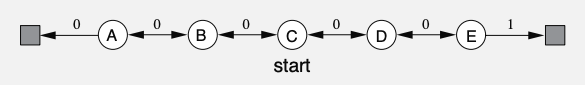
\includegraphics[width=\textwidth]{/ex6.3}
	\caption{Random walk example}
	\label{fig:ex6.3}
\end{figure}

The result of the first episode suggests the episode terminated at the left block for no reward. The value of state $A$ was updated as follows:
\begin{align}
V(A) &= V(A) + \alpha \left[R_{t+1} + V(S_T) - V(A) \right] \\
&= 0.5 + 0.1 \left[0 + 0 - 0.5\right] \\
&= 0.45
\end{align}
$
\hfill \blacksquare
$

\subsection{Exercise 6.4}
\subsubsection{Q}
The specific results shown in the right graph of the random walk example are dependent on the value of the step-size parameter, $\alpha$. Do you think the conclusions
about which algorithm is better would be affected if a wider range of $\alpha$ values were used? Is there a different, fixed value of $\alpha$ at which either algorithm would have performed significantly better than shown? Why or why not?
\subsubsection{A}
It appears from the plot the long-term accuracy of TD methods is inversely proportional to the chosen $\alpha$, which makes sense given larger alphas would cause the value function to oscillate around the true value function. It is not clear from the plot whether different values of $\alpha$ for the MC method would have increased performance as there is no concrete difference in the algorithm performance based on $\alpha$. It appears the main drawback of the monte carlo method is that it makes significantly fewer value function updates than TD methods. For 100 episodes, the MC method can make no more than 100 updates. For the TD method, the expected episode length is 6, and so it makes 600 value function updates in 100 episodes. No value of $\alpha$ can overcome the reduced sample rate.
$
\hfill \blacksquare
$

\subsection{Exercise 6.5}
\subsubsection{Q}
In the right graph of the random walk example, the RMS error of the TD method seems to go down and then up again, particularly at high $\alpha$’s. What could have caused this? Do you think this always occurs, or might it be a function of how the approximate value function was initialized?
\subsubsection{A}
As discussed above, I believe this will always occur for high $\alpha$ as the weight given to the TD error will exaggerate small errors. The will cause the estimated value function to bounce back and forth across the true value without converging. In turn, this will cause the estimate for $V(c)$ (initialised in this example at its true value) to drift away from the correct estimate, increasing RMS error.
$
\hfill \blacksquare
$

\subsection{Exercise 6.6}
\subsubsection{Q}
In Example 6.2 we stated that the true values for the random walk example are $\frac{1}{6}, \frac{2}{6}, \frac{3}{6}, \frac{4}{6}$ and $\frac{5}{6}$ for states A through E. Describe at least two different ways that these could have been computed. Which would you guess we actually used? Why?
\subsubsection{A}
\begin{enumerate}
	\item \textbf{Dynamic Programming}: we know the policy $\pi$ (take either action with $p(a) = 0.5$), and we know the transition function $p(s', r | s, a) = 1 \; \forall s,a $, thus the value of each state can be computed exactly.
	\item \textbf{First-visit monte carlo policy prediction}: set-up the state space and run simulations with our policy $\pi$. After each episode, back-prop the returns to each state and average.
\end{enumerate}

I suspect the authors used dynamic programming as it requires solving 6 trivial simultaneous equations, whereas the MC method may require thousands of episodes to converge on the true value.
$
\hfill \blacksquare
$

\subsection{Exercise 6.7}
\subsubsection{Q}
Design an off-policy version of the TD(0) update that can be used with arbitrary target policy $\pi$ and covering behaviour policy $b$, using at each step $t$ the importance sampling ratio $\rho_{t:t}$ (5.3).
\subsubsection{A}
Our TD update is:
\begin{equation}
V(s) = V(s) + \alpha \left[R_{t+1} + \gamma V(s') - V(s)\right]
\end{equation}
and our importance sampling ratio is:
\begin{equation}
\rho_{t:t} = \frac{\pi(A | S)}{b(A | S)}
\end{equation}

We assume an episode of experience is produced by our behaviour policy $b$, and the update becomes:
\begin{equation}
V_\pi(s) = V_\pi(s) + \alpha \left[\rho_{t:t} R_{t+1} + \rho_{t:t} \gamma V(s') - V(s)\right], 
\end{equation}

i.e. each update is weighted by the likelihood of the action being taken by the target policy compared to the behaviour policy, divided by sum of all previous importance samples.\\
$
\hfill \blacksquare
$
\subsection{Exercise 6.8}
\subsubsection{Q}
Show that an action-value version of (6.6) holds for the action-value form of the TD error $\delta_t = R_{t+1} + \gamma Q(S_{t+1}, A_{t+1}) - Q(S_t, A_t)$, again assuming that the values don’t change from step to step.
\subsubsection{A}
Recall, equation 6.6 was the monte carlo error written in terms of the TD error:
\begin{equation}
G_t - V(S_t) = \sum_{k=t}^{T-1} \gamma^{k-t} \delta_k
\end{equation}

We amend 6.6 as follows:
\begin{align}
G_t - Q(S_t, A_t) &= R_{t+1} + \gamma G_{t+1} - Q(S_t, A_t) + \gamma Q(S_{t+1}, A_{t+1}) - \gamma Q(S_{t+1}, A_{t+1}) \\
&= \delta_t + \gamma \left(G_{t+1} - Q(S_{t+1}, A_{t+1}) \right) \\
&= \delta_t + \gamma \delta_{t+1} + \gamma^2\left(G_{t+2} - Q(S_{t+2}, A_{t+2}\right) \\
\vdots \\
&= \sum_{k=t}^{T-1} \gamma^{k-t} \delta_k
\end{align}
$
\hfill \blacksquare
$

\subsection{Exercise 6.9}
\subsubsection{Q}
Re-solve the windy gridworld assuming eight possible actions, including the diagonal moves, rather than four. How much better can you do with the extra actions? Can you do even better by including a ninth action that causes no movement at all other than that caused by the wind?
\subsubsection{A}
\ProgrammingExercise \\

With the extra actions, the optimal policy is now 7 moves as opposed to 15 moves with 4 actions. Adding the 9th action does not improve the optimal policy, the terminal square is 7 moves away from the start square and so adding an action that keeps the agent stationary cannot improve the policy. See Figures \ref{fig:ex6.9a} and \ref{fig:ex6.9b} plot the optimal policy for 4 and 8 actions respectively. Each agent learned from 10,000 episodes of self-play.
\begin{figure}[h!]
	\centering
	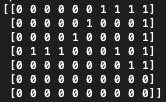
\includegraphics[width=0.5\textwidth]{/ex6.9a}
	\caption{Optimal policy with 4 available actions}
	\label{fig:ex6.9a}
\end{figure}
\begin{figure}[h!]
	\centering
	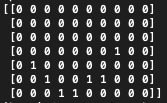
\includegraphics[width=0.5\textwidth]{/ex6.9b}
	\caption{Optimal policy with 8 available actions}
	\label{fig:ex6.9b}
\end{figure}
$
\hfill \blacksquare
$

\subsection{Exercise 6.10}
\subsubsection{Q}
Re-solve the windy gridworld task with King’s moves, assuming that the effect of the wind, if there is any, is stochastic, sometimes varying by 1 from the mean values given for each column. That is, a third of the time you move exactly according to these values, as in the previous exercise, but also a third of the time you move one cell above that, and another third of the time you move one cell below that. For example, if you are one cell to the right of the goal and you move left, then one-third of the time you move one cell above the goal, one-third of the time you move two cells above the goal, and one-third of the time you move to the goal.
\subsubsection{A}
Implementation is identical to above with amended transition function. Exercise not yet completed.
$
\hfill \blacksquare
$

\subsection{Exercise 6.11}
\subsubsection{Q}
Why is Q-learning considered an \textit{off-policy} control method?
\subsubsection{A}
Q-learning is off-policy because the action-selection at $S_{t+1}$ (used for the Q-update) is deterministic i.e. it chooses the greedy action with probability 1. This is in contrast with the behaviour policy used to collect the data which is $\epsilon$-greedy. The policy being updated is therefore different from that being used to collect data, and the algorithm is off-policy.\\
$
\hfill \blacksquare
$

\subsection{Exercise 6.12}
\subsubsection{Q}
Suppose action selection is greedy. Is Q-learning then exactly the same algorithm as SARSA? Will they make exactly the same action selections and weight updates?
\subsubsection{A}
If action-selection is greedy, the algorithms become identical, but the action selections and weight updates may differ depending on the arbitrary initialisation of $Q$ and $S$. For example, if each state-action pair is assigned a random value $Q(S, A) \in (0,1]$, the greedy action selection in each case will differ. Because action selection differs, updates differ, and because neither algorithm explore, there is no guarantee they will converge on the same solution.
$
\hfill \blacksquare
$

\subsection{Exercise 6.13}
\subsubsection{Q}
What are the update equations for Double Expected Sarsa with an $\epsilon$-greedy target policy?
\subsubsection{A}
Instead of taking the maximum action over $Q$, we continue to follow our $\epsilon$-greedy behaviour policy. The expected sarsa update is:
\begin{equation}
Q(S_t, A_t) \leftarrow Q(S_t, A_t) + \alpha \left[R_{t+1} + \gamma \sum_{a} \pi(a | S_{t+1}) Q(S_{t+1}, a) - Q(S_t, A_t) \right] \\
\end{equation}
Therefore our updates become:
\begin{align}
Q_1(S_t, A_t) &\leftarrow Q_1(S_t, A_t) + \alpha \left[R_{t+1} + \gamma \sum_{a} \pi(a | S_{t+1}) Q_2(S_{t+1}, a) - Q_1(S_t, A_t) \right]  \\
Q_2(S_t, A_t) &\leftarrow Q_2(S_t, A_t) + \alpha \left[R_{t+1} + \gamma \sum_{a} \pi(a | S_{t+1}) Q_1(S_{t+1}, a) - Q_2(S_t, A_t) \right]
\end{align}
with our policy $\pi$ being $\epsilon$-greedy.
$
\hfill \blacksquare
$

\subsection{Exercise 6.14}
\subsubsection{Q}
Describe how the task of Jack’s Car Rental (Example 4.2) could be reformulated in terms of afterstates. Why, in terms of this specific task, would such a reformulation be likely to speed convergence?
\subsubsection{A}
In Jack's car rental example we each location can hold cars in the range (0,20). Up to 5 cars can be moved from one location to the other overnight to accommodate expected sales, taking one of these actions will move us deterministically to a new state. If there was uncertainty in how we transition between states, it makes sense to learn a conventional value function that probabilistically accounts for this uncertainty, but given the transition is certain, we can learn the afterstates (the states from which we will sell the cars in the morning) and proceed.

We speed convergence by reducing the number of states to be evaluated. For example, if our state in the evening is five cars at each location: $(5,5)$ and our action is to move one car to the second location such that our morning state becomes $(4,6)$, we can evaluate this state as the same as the state-action pair of $(4,6)$ and choosing to move no cars.
$
\hfill \blacksquare
$
	
\end{document}